\documentclass[UTF8]{ctexbook}

\usepackage{scigeneral}
% SCI book 的模板 sty,适用于中文
\usepackage{scibookchn}

\interfootnotelinepenalty=10000

\title{王新龙声学博文}

% start each section on a new page
% \let\stdsection\section
% \renewcommand\section{\newpage\stdsection}

\begin{document}

\maketitle

\tableofcontents

\chapter{声波的基本性质}
\section{流体力学引论}

\emph{摘要}\ 流体之声是流体质点振动形式和能量的传递。
所以,声学与流体动力学存在某种程度的相关性。
欲精通声学理论,必先掌握必要的流体力学基本知识和基本理论。
无奈在教学实践中发现,仍有不少学生阙如,一定程序上影响了《声学基础》课的
学习进程。
监于此,本文简介理想流体的流体力学基本理论,以期作为读者钻研声学的预备。

\emph{正文}\ 流体包括气体和液体,可流动而固定形状(除非置于固定形状的容器之内)。
尽管流体由微观上离散的分子或原子组成,但流体力学仅研究流体的宏观力学现象。
所以,流体力学把流体视若宏观连续的媒质。
流体力学的理论分析涉及到流体的「体积元」概念。
所谓体积元,概指宏观无限小但微观可包含大量流体分子(或原子)者。
宏观无限小意谓体积元内宏观物理量几乎是均匀,因此可描述体积元所在空间的「点」
的流体状态。
另一方面,这些物理量必须具有统计物理的意义,因此微观上必须足够大,以包含
大量分子(或原子),也即,体积元的尺寸必须远大于分子的平均自由程。
\emph{体积元是纯空间概念},与之相关但相异的概念是流体的「质点」。
所谓质点(particle),其实也是如此这般的流体体积元,但\emph{
	质点是流体的微实体,
具有质量},可视为流体的宏观「分子」(犹如可变形的流体微粒)。
无数质点的运动遂构成了流体的运动。

本文仅考察理想液体,即无黏性、无热导损耗(绝热)的流体。

\subsection{流场描述}
三维流体空间中,每个流体质点在每个时刻$t$均有其可观测的确定位置,用位置
矢量$\vb{r}$描述。
在Cartesian坐标系中,$\vb{r}=(x,y,z)$,其中$x$、$y$和$z$是$\vb{r}$在此坐标
系中的三个分量。
显然,某质点的位置矢量$\vb{r}$不仅随时而变,而且取决于其初始时刻$t=t_0$的
位置$\vb{R}=(a,b,c)$,即$\vb{r}$是初始位置$\vb{R}$和时间$t$的多元函数:
\begin{equation}
	\vb{r} = \vb{r}(\vb{R},t)\qor 
	\begin{dcases}
		x&=x(a,b,c,t)\\
		y&=y(a,b,c,t)\\
		z&=z(a,b,c,t)
	\end{dcases}
\end{equation}

流速$\vb{v}$是流体质点的运动速度(velocity),定义为质点位置矢量$\vb{r}$
的时间变化率:
$$\vb{v}=\dv{\vb{r}}{t} = \qty(\dv{x}{t}, \dv{y}{t},\dv{z}{t}) =
\vb{v}(\vb{R},t)$$

在直角坐标系中,$\vb{v}=\qty(v_x,v_y,v_z)$具有3个分量:
$v_x = \dv*{x}{t}$、$v_y=\dv*{y}{t}$和$v_z=\dv*{z}{t}$。
与位置矢量$\vb{r}$一样,流速$\vb{v}$也是初始位置$\vb{R}$和时间$t$的函数。
流速描述了流体的运动状态。
除此之外,尚需诸如压力$P$(pressure)、密度$\rho$(density)、温度$T$
(temperature)等其它物理量,以全面描述流体的状态。
然而,根据热力学(thermodynamics)理论,\emph{一般仅需两个独立的热力学状态
	变量即可完全描述流体的热力学状态},余者悉可经状态方程确定。

上述这种描述中,流体的状态物理量表为质点初始位置$\vb{R}$和时间$t$的函数:
\begin{subequations}
\begin{align}
		\vb{v} = \vb{v}(\vb{R},t)\qc P = P(\vb{R},t)\qc \rho = \rho(\vb{R},
		t),\label{eq:fluid_v_a}\\
		\label{eq:fluid_v_b}
		\vb{v} = \vb{v}(\vb{r},t)\qc P = P(\vb{r},t)\qc \rho = \rho(\vb{r},
		t)
\end{align}
\end{subequations}
这种描述方法在流体力学中被称为拉格朗日描述(Lagrange description)。
\emph{Lagrange描述视流体的运动为无数质点运动的集合,并试图「跟踪」(trace)
	每一个质点的轨迹(trajecotry)。}
这种描述体现了机械运动的确定论观(determinism),一旦测得某质点在某时刻的位
置$\vb{R}$及其状态信息,则该质点在任意时刻$t$的状态性质尽可通过式(\ref{eq:fluid_v_a})获知。
时刻$t=t_0$的位置矢量$\vb{R}$不仅作为每个流体质点的「标记」,而且也作为
Lagrange描述体系下的坐标。
因$\vb{R}$其实是流体质点的初始位置,故在Lagrange坐标系中状态量对时间的全
导数(full derivatives)等同于时间偏导数(partial derivatives),例如:
$$\dv{t} \vb{r}(\vb{R},t) = \pdv{t} \vb{r}(\vb{R},t)\qc 
\dv{t} \vb{v}(\vb{R},t) = \pdv{t} \vb{v} (\vb{R},t)$$

比之Lagrange描述,Euler描述在流体力学中更常用、更方便。
\emph{Euler描述重在当前$t$时刻流体状态在空间$\vb{r}$的分布},即式(\ref{eq:fluid_v_a})。
所以,这是一种场(field)---流场---的描述方法。
\emph{在此描述中,位置矢量$\vb{r}$仅被视为与时间完全无关的独立变量。}
然而,追根溯源,位于$\vb{r}$处的流体质点是初始时刻$t_0$从$\vb{R}$处迁移而
来,即$\vb{r}=\vb{r}(\vb{R},t)$,故而上述两种描述以如下方式关联:
\begin{equation}
	\begin{dcases}
		\vb{v}(\vb{R},t) & = \vb{v}\qty(\vb{r}(\vb{R},t),t)\\
		{P}(\vb{R},t) & = P\qty(\vb{r}(\vb{R},t),t)\\
		{\rho}(\vb{R},t) & =\rho\qty(\vb{r}(\vb{R},t),t)\\
	\end{dcases}
\label{eq:fluid_correlation}
\end{equation}
因此两种描述,就有两种不同意义的状态变量时间变化率。
其一是\emph{(被视作流体微粒的)质点的状态时间变化率,即Lagrange描述下的时间变化率。}
它反映了质点本身在其运动过程中的时间变化,质点速度(流速)$\vb{v}$即为典型。
其二是\emph{空间某固定点$\vb{r}$的时间变化率,即Euler描述下的时间偏导数},例如:
$$
\pdv{t}\vb{v}(\vb{r},t)\qc 
\pdv{t}P(\vb{r},t)\qc 
\pdv{t}\rho(\vb{r},t)
$$
其中,位置矢量$\vb{r}$被视为独立的空间变量,与时间无关。
其实,这两种时间变化率分别是Lagrange和Euler描述下状态量的时间导数。

两种时间变化率是相互关联的。
观察式(\ref{eq:fluid_correlation})便知,\emph{Lagrange描述下的时间变化率
等于Euler描述下的时间全导数}(专用微分符号$\dv*{t}$表示之)。
所以,欲求Euler描述下的Lagrange意义下的时间变化率,求时间导数时必须顾及
空间变化量$\vb{r}=(x,y,z)$本身是时间的函数。比如,
\begin{align*}
	\dv{t} \rho(\vb{r},t) & = \pdv{t}\rho (\vb{r},t)+\dv{x}{t} \pdv{x}
	\rho(\vb{r},t) +\dv{y}{t} \pdv{y} \rho(\vb{r},t)+\dv{z}{t} \pdv{z} \rho
	(\vb{r},t)\\
	&=\pdv{t}\rho(\vb{r},t) + (\vb{v}\vdot \grad)\rho(\vb{r},t)\\
	&=\qty(\pdv{t} + \vb{v}\vdot \grad )\rho (\vb{r},t)
\end{align*}
式中,三维梯度算符
$$\grad \equiv \qty(\pdv{x}, \pdv{y}, \pdv{z})$$
由此可见,在Euler描述的时间全导数与偏导数存在如下的微分算符关系
\begin{equation}
	\dv{t} = \pdv{t} + \vb{v}\vdot \grad
	\label{eq:fluid_dt}
\end{equation}
等式右端的第一项是空间固定点的导数,称为\emph{本地时间导数}(即Euler描述
下的时间变化率);而第二项是流动而产生的时间变化率贡献,称为\emph{对流导数}。


\subsection{理想流体运动的基本方程}
\subsubsection{连续性方程}
设$V$是流体空间某任意(但大小形状固定)的体积,其中所含流体的质量是
$$\iiint_V \rho(\vb{r},t)\dd x \dd y \dd z$$
盖因流动,流体必经$V$的封闭曲面$S$流入或流出。
考察$S$上的某有向面元$\dd \vb{S} = \vb{n} \dd S$其中$\vb{n}$是$\dd \vb{S}$
面元的单位法向矢量。
单位时间内经$\dd \vb{S}$流出的流体体积是$(\vb{v}\vdot \vb{n}) \dd{S}=
\vb{v}\vdot \dd \vb{S}$,故流出的质量是$\rho \vb{v}\vdot \dd \vb{S}$。
对整个封闭曲面$S$积分,
$$\oiint_S \rho\vb{v}\vdot \dd \vb{S}$$
就得到单位时间内经封闭表面$S$流出的质量(面积分值为正表示净流出的流体,为
负表示净流入的)。
被各函数$\rho \vb{v}$是一个矢量,谓之流体的质量能量密度矢量,其方向与流速
$\vb{v}$一致,其量值等于单位时间内流经与流速$\vb{v}$相垂直的单位面积的流体
质量。
除了质量能量密度矢量之意外,$\rho \vb{v}$还具有单位体积流体动量之意(见下文
动量守恒部分)。
根据质量守恒定律,若体内元流源,则经边界$S$流出的质量必然导致单位时间内$V$
内质量的减少,即
$$\oiint_S \rho \vb{v}\vdot \dd{\vb{S}} = -\pdv{t} \iiint_V \rho \dd x\dd
y\dd z$$
等式右端的时间偏导数意谓单位时间内的增长率,而前面取负号则表示减小率。
前已假定,体积$V$在空间固定,故右端的时间导数可直接移入体积分号内。
进一步对左端的封闭曲面积分应用Gauss定理,并合并俩积分,则上式化为如下体
积分:
$$\iiint_V\qty[\pdv{\rho}{t} +\div{(\rho\vb{v})}]\dd x \dd y \dd z=0$$

因体积$V$大小任意,故体积分下的被积函数必等于零:
\begin{subequations}
	\begin{align}
		\pdv{\rho}{t} +\div(\rho\vb{v}) & = 0,\\
		\dv{\rho}{t} + \rho \div\vb{v} &= 0,\label{eq:fluid_continuityB} \\
		\pdv{\rho}{t} + \div (\rho \vb{v}) & = \rho q(\vb{r},t)\label{eq:fluid_continuityC}
	\end{align}
	\label{eq:fluid_continuity}
\end{subequations}
此即质量的连续性方程,通常谓之\emph{连续性方程}(equation of continuity)。
可见,连续性方程是质量守恒定律之数学表述。
应用人气周知的散度公式:$\div (\rho\vb{v}) = \vb{v} \vdot \grad \rho +
\rho \div{\vb{v}}$,并把算符公式(\ref{eq:fluid_dt})应用于密度$\rho$的时间
导数,则连续性议程也可写成如式(\ref{eq:fluid_continuityB})的等价形式。

易把连续性方程(\ref{eq:fluid_continuity})推广到有质量产生的情形。
设单位体各的流体在单位时间内产生的流体质量是$\rho q(\vb{r},t)$($q$是流体
的体积生成率),则根据质量守恒定律不难导出式(\ref{eq:fluid_continuityC})。


\subsubsection{Euler方程}
仍考虑固定形状大小的流体体积$V$。
若无其它外力,则作用在此体积上的外力仅仅是在包围$V$的封闭曲面$S$上所受的压力
的总和:
$$-\oiint_S P\dd\vb{S} = -\iiint_V \grad P \dd x \dd y \dd z$$
其中的等式已经利用了针对标量的封闭曲面面积分Gauss定理。
须注意,流体的压力总与边界面的外法向相反,垂直界面指向流体内部,故上式取
负号。
上式的等式表明,单位体积的流体质点受到压力:$-\grad P$。
而单位体积的流体质点的质量是$\rho$,所以根据牛顿第二定律得到如下运动方程
(equation of motion)
\begin{equation}
	\rho \dv{\vb{v}}{t} = -\grad P
	\label{eq:fluid_eulera}
\end{equation}
其Cartesian坐标的分量形式
$$\rho \dv{v_x}{t} = -\pdv{P}{x}\qc \rho \dv{v_y}{t} = -\pdv{P}{y}\qc
\rho \dv{v_z}{t} = -\pdv{P}{z}$$
再次强调,因牛顿定律是针对质点而言的,上式左端的流速导数是质点的加速度,即
流速$\vb{v}$的时间全导数。
根据全导数与偏导数的关系式(\ref{eq:fluid_dt}),运动议程又可表达成
\begin{equation}
	\pdv{\vb{v}}{t} +\vb{v}\vdot \grad \vb{v} = -\frac1\rho \grad P
	\label{eq:fluid_eulerb}
\end{equation}
式中流速$\vb{v}$的梯度
$$\grad \vb{v} \equiv \qty(\pdv{\vb{v}}{x}, \pdv{\vb{v}}{y},\pdv{\vb{v}}{z})
$$
是矢量的矢量 --- --- 张量,具有9个分量。
或者,方程(\ref{eq:fluid_eulerb})也可以写成分量的形式
$$
\begin{dcases}
	\pdv{v_x}{t} + \vb{v}\vdot \grad v_x&=-\frac1\rho \pdv{P}{x},\\
	\pdv{v_y}{t} + \vb{v}\vdot \grad v_y&=-\frac1\rho \pdv{P}{y},\\
	\pdv{v_z}{t} + \vb{v}\vdot \grad v_z&=-\frac1\rho \pdv{P}{z}
\end{dcases}
$$
此方程由Euler于1755年首次提出,是谓Euler方程(Euler Equation)。


如果单位质量的流体还受到外力$\vb{g}$的作用,则Euler方程(\ref{eq:fluid_eulerb})
右端尚需加上单位体积的外力$\rho \vb{g}$。
两端均除以密度$\rho$,得到
\begin{equation}
	\pdv{\vb{v}}{t} + \vb{v}\vdot \grad \vb{v} =-\frac1\rho \grad P + \vb{g}
	\label{eq:fluid_eulerc}
\end{equation}
若所受外力是重力,则$\vb{g}=-g\vu{e}_z$,其中$g$是重力加速度,$\vu{e}_z$
指沿水平面垂直向上的单位矢量

\subsubsection{状态方程}
前已阐述,流体的状态不仅包括运动状态($\vb{v}$),还包括诸如压力$P$、密度
$\rho$等热力学状态量。
设单位质量流体(或质点)的熵为$s$。
熵$s$可表为压力$P$和密度$\rho$的状态函数:
$$s = s(P,\rho)$$
绝热过程不存在热量交换,故流体的熵守恒,其数学表示为:
\begin{equation}
	\dv{s}{t} = 0
	\label{eq:fluid_sa}
\end{equation}
或根据公式(\ref{eq:fluid_dt}),有
\begin{equation}
	\pdv{s}{t} +\vb{v}\vdot \grad s = 0
	\label{eq:fluid_sb}
\end{equation}
方程(\ref{eq:fluid_sa})表明,$s(P,\rho)=$常数,即流体的绝热过程是\emph{等
	熵运动}。
从中原则上可求得函数关系:
\begin{equation}
	P=P(\rho)
\end{equation}

设流体的温度为$T$,单位质量流体的焓为$h$。
根据热力学的基本关系:
\begin{equation}
	\dd h = T\dd s + \frac1\rho \dd{P}
\end{equation}

可知,对于等熵运动($\dd s=0$),存在如下关系:
\begin{equation}
		\dd h = \frac1\rho \dd{P}
		\imp \grad h  = \frac1\rho \grad P\qc \qty(h=\int \frac{\dd P}{\rho}
		)
\end{equation}

同时,应用矢量分析公式\footnote{
矢量公式
$$\frac12 \grad (\vb{v}\vdot \vb{v}) = \vb{v}\cp \qty(\curl \vb{v}) + 
\qty(\vb{v}\vdot \grad)\vb{v}$$
等式两端点积流速$\vb{v}$,并考虑到$\vb{v}\cp (\vb{v}\cp \vb{A}) = 0$(
$\vb{A}$任意),遂有
$$\frac12 \vb{v} \vdot \grad v^2 =   \vb{v}\vdot \qty(\vb{v}\vdot
\grad)\vb{v}$$
其中$v^2=\vb{v}\vdot \vb{v}$。},
则可把Euler方程(\ref{eq:fluid_eulerb})表达成:

\begin{equation}
	\pdv{\vb{v}}{t} +\grad \qty(\frac12 \vb{v}\vdot \vb{v} + \int\frac{
	\dd P}{\rho} ) = \vb{v}\times\qty(\curl \vb{v})
\end{equation}

以上导出了Euler描述下理想流体的连续性方程(\ref{eq:fluid_continuity})、
Euler(运动)方程(\ref{eq:fluid_eulera})(\ref{eq:fluid_eulerb})(\ref{eq:fluid_eulerc}),并简述了
热力学状态方程(\ref{eq:fluid_sa})(\ref{eq:fluid_sb})。
这些方程构成了Euler描述体系下理想流体的基本方程。
至于基Lagrange描述的形式,参见《流体运动的Lagrange描述》一文。

\subsection{动量和能量的连续性方程}
\subsubsection{动量守恒}

在连续性方程(\ref{eq:fluid_continuity})的两端乘以速度$\vb{v}$的$x$分量
$v_x$,再与Euler方程(\ref{eq:fluid_eulera})的$x$分量相加,得到
\begin{equation}
	\pdv{(\rho v_x)}{t} + \div \qty[(\rho v_x)\vb{v}] = -\pdv{P}{x}
	\label{eq:fluid_momentuma}
\end{equation}
为明了此方程的物理意义,特对此方程两端作被变截面$S$包围的任意体积$V$的体
积分,
\[
	\pdv{t} \iiint_V \rho v_x \dd x \dd y \dd z +
	\oiint_S \rho v_x \qty(\vb{v} \vdot \dd \vb{S}) 
	= -\iiint_V \pdv{P}{x} \dd x \dd y \dd z
\]
其中等式左端的第二项面积分是利用Gauss定理的结果。
若应用标量的Gauss定理,则等式右端实际上是
$$
	-\iiint_V \grad P \dd x \dd y \dd z
	= -\oiint_S P \dd \vb{S}
$$
的$x$方向分量。
因此,上列微分方程等价于如下的积分方程,
$$
	\pdv{t}\iiint_V \rho v_x \dd x \dd y \dd z
	=-\oiint_S \rho v_x \qty(\vb{v}\vdot \dd \vb{S}) - \qty(\oiint_S
	P \dd \vb{S})_x
$$
其中最后一项的括号外的下标表示$x$分量。
方程左端的被积函数$\rho v_x$乃单位体积的流体动量在$x$方向的投影,而其体积分就是
$V$内流体总却是在$x$方向的分量;
右端第一个面积分是单位时间内经封闭曲面$S$流入的$x$方向动量,而第二个压力面积分是
作用在$V$上的$x$方向总压力分量。
因此,上列积分方程正是$x$分量动量守恒定律的积分表述,而方程(
\ref{eq:fluid_momentuma})是$x$方向动量守恒的微分表述。
同理,可以得到对应$y$和$z$分量的积分方程。
合并三个分量积分方程,得到矢量形式的动量守恒积分方程表示,
$$
	\pdv{t}\iiint_V \rho \vb{v} \dd x \dd y\dd z = 
	-\oiint_S \rho \vb{v} \qty(\vb{v} \vdot \dd \vb{S})
	-\oiint_S P\dd\vb{S}
$$
方程左端的被积函数$\rho \vb{v}$乃单位体积的流体动量,而其体积分就是$V$
内流体的总动量;
右端第一个面积分是单位时间内经封闭曲面$S$流入的动量,而第二个压力面积分是
作用在$V$上的总压力。
对应的微分形式是
\begin{equation}
	\pdv{t} \qty(\rho \vb{v}) +
\end{equation}

TBD


\section{声学量的复数运算\\
Complex Operations for Acoustical Quantities}

\emph{摘要}\ 振动与声学量虽然是可观测的实数物理量,但也可用复数表示。
复数表示不但可极大地简化数学演算,因此无论在线性还是非线性的声学理论中均
广泛采用复数表示声学量。本文简述声学量的复数表示及运算规则,并举例说明。

设小写的$x$为实数量,而大写的$X$为对应的复数量,即$x=\Re(X)$,其中
$\Re(X)$表示取复数量$X$的实部,即
$$
x = \Re(X) = \frac12(X+X^*)
$$
其中右上标的星号「*」表示复共轭操作。显然,实数量$x$与其对应的复数量$X$并非
一一对应。复数量$X$加上任意的线虚数$\mj y$并不影响其意义:
$$
x = \Re(X) = \Re(X+\mj y)
$$

\subsection{加法规则}
若$x$、$y$和$z$为实数量,$a$和$b$是任意的实数,$z=ax+by$。设$x$、$y$和$z$
对应的复数量分别为$X$、$Y$和$Z$,即$x=\Re(X)$、$y=\Re(Y)$和$z=\Re(Z)$,则
因
$$
z = ax+by = \Re(aX+bY) = \Re(Z)
$$
所以,复数量$X$、$Y$和$Z$之间存在以下关系
$$Z=aX+bY$$
现设$x$是时间$t$的函数:$x=x(t)$。它对应的复数量$X$也是时间的函数:$X=
X(t)$。由于导数和积分本质上是线性加法去处,因此存在关系:
$$\dv{t} \Re(X) =\Re\qty(\dv{X}{t})\qc \int \Re(X) \dd{t} = \Re 
\qty(\int X\dd{t})$$

即复数$\dv*{X}{t}$是实数量导数$\dv*{x}{t}$对应的复数量,复数积分$\int X
\dd{t}$是实数积分$\int x\dd{t}$对应的复数量。

\subsection{乘法规则}
现设$z$是$x$和$y$之积,$z=xy$,对应的复数量为$Z$。根据定义,
$$z=xy =\Re(X)\Re(Y) = \Re(\Re(X)Y)=\Re(X\Re(Y))$$
所以,
\begin{subequations}
	\label{eq:complexop_Z}
	\begin{equation}Z= \Re(X)Y = \frac12 (XY+X^*Y)\end{equation}
	\begin{equation}Z=X\Re(Y) = \frac12 (XY+XY^*)\end{equation}
\end{subequations}
再次申明,式(\ref{eq:complexop_Z})中两个表式所给出的$Z$在数学上严格而言是
不等的,只因$Z$的实部才有物理意义,故两种表示在物理上等价。

\subsection{时间简谐量的周期平均值}
复数表示对于简谐声学量的计算尤其有效。假设与时间$t$的依赖关系为$\exp(\mj 
\omega t)$,其中$\omega = 2\uppi /T$为频率,$T$是振动周期,$\mj$是虚数单位
。例如,$X$和$Y$是时间简谐的复量
$$X=X\subt{a} \me^{\mj \omega t }\qc Y = Y\subt{a}\me^{\mj \omega t}$$
其中,$X\subt{a}$和$Y\subt{a}$分别为$X$和$Y$的复振幅,是与时间$t$无关的常数。
则有
$$\dd{X}{t}=\mj \omega X\qc \int X\dd{t} = \frac{X}{\mj \omega}$$
根据(\ref{eq:complexop_Z}),此时乘积$z=xy$的复数表达式为
$$Z=\frac12 X\subt{a}^* Y\subt{a}+\frac12 X\subt{a}Y\subt{a}\me^{2\mj \omega t}$$
上式第二项有时间依赖关系$\exp(2\mj \omega  t)$,描述了乘积量$z$的瞬态运动。
这是一个二次谐波(频率$2\omega$),其周期平均为零。第一项是与时间无关的
「直流」项,等于复量$Z$的周期平均值:
$$\bar{Z} = \frac1T \int_0^T Z(t) \dd{t} = \frac12 X\subt{a}^* Y\subt{a} =
\frac12 X^* Y$$
所以,乘积量$z=xy$的周期均值为
$$\bar{z}=\frac1T \int_0^T z\dd{t} = \overline{\Re(Z)} = \Re(\bar{Z})
=\frac12\Re(X^*Y)$$
即,存在以下重要的乘积平均法则
\begin{equation}
	\overline{x(t)y(t)} = \frac12 \Re(X^*Y) \label{eq:complexop_xy}
\end{equation}
对于简谐振动而言,振动物理量本身的时间均值往往为零。但如振动量的乘积等非
线性运算,多产生类似的「直流」项,因而平均值非零。\emph{「直流」和高次谐波
的产生为典型的非线性效应。}

以下以若干典型振动与声学量为例,说明复数运算的应用。

\subsubsection{单振子周期平均能量}
设有质量为$M\subt{m}$、弹性系数为$K\subt{m}$的单振子,其质点的位移为$x$,速度
$v$,对应的复位移为$X$,复速度为$V$。单振子的势能和动能分别为
$$E\subt{p} = \frac12 K\subt{m} x^2 = \frac12 K\subt{m}\qty[\Re(X)]^2$$
$$E\subt{k} = \frac12 M\subt{m} v^2 = \frac12 M\subt{m} \qty[\Re(V)]^2$$
若单振子仅作简谐振动,则根据式(\ref{eq:complexop_xy}),势能和动能的一个周期
平均值分别为
$$\overline{E\subt{p}} = \frac12 K\subt{m} \overline{x^2} = \frac14 K\subt{m}
|X|^2$$
$$\overline{E\subt{k}} = \frac12 M\subt{m} \overline{v^2} = \frac14 M\subt{m}
|V|^2$$
对于自由振动,
$$V = \mj \omega_0 X\qc \qty(\omega_0 = \sqrt{\frac{K\subt{m}}{M\subt{m}}})$$
代入前式,知平均势能等于平均动能:
$$\overline{E\subt{p}} = \overline{E\subt{k}}$$

\subsubsection{声能通量密度和声强的运算}
声能通量密度$\vb{I}$为声压$p$与速度适量$\vb{v}$的乘积:$\vb{I}=p \vb{v}$。
声压、速度和声能通量密度等物理量本身是实量,但均可以用复数表示。在振动
与声的问题中,极大部分情形下所涉及的是复数量及其运算,因此在下文中我们放弃
前面用大写字母表示复量的做法,而一概约定:除非特别说明,\emph{所有的变量符号
均表示对应实量的复量},如声压、复速度和复能量通量密度仍用$p$、$\vb{v}$和
$\vb{I}$表示;如果确实需要用到实数量,则只要对这些复数量取实部操作$\Re$即可
。例如,根据公式(\ref{eq:complexop_Z}),复声能通量密度的公式可写成
\begin{equation}
	\label{eq:complexop_I}
	\vb{I} = \frac12 p\vb{v} + \frac12 p^* \vb{v}
\end{equation}
取实部$\Re(\vb{I})$即为实声能通量密度。

对频率为$\omega$的简谐声波,公式(\ref{eq:complexop_I})的第一项描述声能通量
密度之瞬变,而第二项是「直流」分量,为复声能通量密度之时间均值:
\begin{equation}
	\label{eq:complexop_barI}
	\overline{\vb{I}} = \frac1T \int_t^{t+T}\dd{t} = \frac12 p^* \vb{v}
\end{equation}
取其实部即得到\emph{声强}:
$$\Re(\overline{\vb{I}}) = \frac12 \Re\qty(p^* \vb{v})$$
可见,采用复运算,易分离场量(此处是声能通量密度)的时变和时不变成份。

对于平面行波,传播方向为$\vb{n}$(单位矢量),则媒质质点的振速$\vb{v}
=(p/z_0)\vb{n}$,代入公式(\ref{eq:complexop_I})和(\ref{eq:complexop_barI})
得到
$$\vb{I} = \frac{1}{2z_0}\qty(p^2+|p|^2)\vb{n}$$
$$\overline{\vb{I}} = \frac{1}{2z_0} \overline{\qty(p^2+|p|^2)}
=\frac{|p|^2}{2\rho_0 c_0 }\vb{n}$$
式中$z_0=\rho_0c_0$是媒质的声特性阻抗率。

\subsubsection{声能密度复数运算}
对平面波而言\footnote{编著添加。},用实声学量表示的流体声场的(瞬时)声能
密度为
$$\eps = \frac12 \rho_0 \qty[\vb{v} \vdot \vb{v} +\qty(\frac{p}{z_0})]$$
其中的声压$p$和速度$\vb{v}$是实数量。若全改用复量表示,且仍采用相同的变量
符号,则上式应改为
\begin{align}
	\label{eq:complexop_eps}
	\eps & = \frac14 \rho_0 \qty[(\vb{v}\vdot\vb{v} + \vb{v}^*\vdot
	\vb{v}) +\frac{1}{z_0^2} \qty(p^2+p^* p)]\nonumber\\
	& = \frac14 \rho_0 \qty[\vb{v}\vdot\vb{v}+ \qty(\frac{p}{z_0} )^2]
	+\frac14 \rho_0 \qty(\vb{v}^*\vdot \vb{v} + \qty|\frac{p}{z_0}|^2)
\end{align}
对频率$\omega$的简谐声波,公式(\ref{eq:complexop_eps})后一等式中的第一项描述
声能密度的瞬时变化,而第二项是「直流」分量,为复声能密度之时间周期平均值,
取其实部即为平均声能密度。因此,简谐声场的平均声能密度为
\begin{equation}
	\label{eq:complexop_bareps}
	\overline{\eps} = \frac14 \rho_0 \qty(|\vb{v}|^2 +\frac{|p|^2}{z_0^2})
\end{equation}

对于沿方向$\vb{n}$传播的平面行波,把$\vb{v}=(p/z_0)\vb{n}$代入公式
(\ref{eq:complexop_eps})和(\ref{eq:complexop_bareps})得到
\begin{align*}
	\eps &= \frac{1}{2\rho_0c_0^2} (p^2+|p|^2)\\
	\overline{\eps} &= \frac{1}{2\rho_0c_0^2} |p|^2
\end{align*}


\section{全反射状态的声场与声能流}
英文标题:
Sound Fields and Energy Flux Under Total Reflection

Web:
http://xlwangnu.blog.163.com/blog/static/190719270201192502043374/

\emph{摘要}
全反射是常见声光现象。在媒质交界面上,若入射媒质的声速不如透射媒质的(或折
射率小于1),则当入射角足够大就会发生全反射,入射声能悉数反射。虽然如此,
全反射下声场如何分布?透射媒质中是否存在声场?如存在,取何种波动方式?此
正本文试图回答的问题。分析表明,在全反射下,(1)入射媒质中的总声场在界面法
向呈驻波形式,而在界面切向呈行波形式;(2)仍存在透射声波,但以沿界面传播的
表面波形式存在,但垂直于界面的方向上指数衰减。

若透射媒质的声速$c_2$大于入射媒质的声速$c_1$,且入射角(incident angle)
$\theta\subt{i}$大于全反射临界角$\theta\subt{ic}$,
\begin{equation}
\theta\subt{ic} = \arcsin \frac{c_1}{c_2} = \arcsin n, \qty(n=\frac{c_1}{c_2}
<1)
\end{equation}
声波全部反射。此即著名的\emph{声全反射现象}(total reflection)。与光
的全反射略有不同,声的全反射一般发生在“硬界面”,如从空气到水,从水到固体。
光的全反射则发生在“软表面”---从光密介质入射到光疏介质,如光纤内的光反射,故
而一般称之为全内反射(Total internal reflection)。或问:在全反射状态,声场
分布如何?声能如何传播?此正本文所欲讨论的。

\subsection{声场分布}
如图xx所示,频率为$\omega$的平面声波从声特性阻抗率为$\rho_1c_1$的媒质中以角
度$\theta\subt{i}$入射到声特性阻抗率为$\rho_2c_2$的媒质上。
设入射方向和两媒质边界面的法向构成的平面为$(x,y)$平面,$x$轴沿边界内法向,
$y$轴在边界平面上。根据平面行波论,入射(incident)、反射(reflected)和
透射(transmitted)的声场解各具如下形式:
\begin{equation}
	\label{eq:totalref_pressure}
	\begin{cases}
	p\subt{i} = p\subt{ia} \me^{-\mj k_1 \vb{n}\subt{i} \vdot \vb{r}}
	\qc \vb{v}\subt{i} = \dfrac{p\subt{i}}{\rho_1c_1} \vb{n}\subt{i}\\
	p\subt{r} = p\subt{ra} \me^{-\mj k_1 \vb{n}\subt{r} \vdot \vb{r}}
	\qc \vb{v}\subt{r} = \dfrac{p\subt{r}}{\rho_1c_1} \vb{n}\subt{r}
	\qc (p\subt{ra} = r_p p\subt{ia}) \\
	p\subt{t} = p\subt{ta} \me^{-\mj k_2 \vb{n}\subt{t} \vdot \vb{t}}
	\qc \vb{v}\subt{t} = \dfrac{p\subt{t}}{\rho_2c_2} \vb{n}\subt{t}
	\qc (p\subt{ta} = t_p p\subt{ta}) 
	\end{cases}
\end{equation}
式中,$p\subt{ia}$、$p\subt{ra}$和$p\subt{ta}$分别为入射、反射和透射(折射)
波的声压幅度,$r_p$和$t_p$分别为声压反射系数和透射系数,$\theta\subt{t}$为
折射角(refracted angle),$k_1$和$k_2$分别为入射和透射媒质的波数,
而$\vb{n}\subt{i}$、$\vb{n}\subt{r}$和$\vb{n}\subt{t}$则依次为入射、反射和
折射波的方向矢量,
\begin{equation}
	\label{eq:totalref_n}
	\vb{n}\subt{i}=(\cos \theta\subt{i}, \sin \theta\subt{i})\qc 
	\vb{n}\subt{r}=(-\cos \theta\subt{r}, \sin \theta\subt{r})\qc 
	\vb{n}\subt{t}=(\cos \theta\subt{t}, \sin \theta\subt{t})
\end{equation}
在$\vb{n}\subt{r}$表达式中,已利用了关系$\vb{theta}\subt{r}=\theta\subt{i}$。为
简洁起见,本文一根省略时间因子$\exp(\mj \omega t)$。

根据Snell定律(折射律),
\begin{equation}
	\label{eq:totalref_snell}
	\sin\theta\subt{t} = \frac{\sin\theta\subt{i}}{n}\qc (n<1)
\end{equation}
当$\theta>\theta\subt{ic}$时,$\sin\theta\subt{t}>1$,$\theta\subt{t}$不复为实数
而是复数。是以,作复变换:$\theta\subt{t} \rightarrow \psi$,
\begin{equation}
	\label{eq:totalref_theta_trans}
	\theta\subt{t} = \frac{\uppi}{2}+\mj \psi\qc 
	\begin{cases}
		\sin \theta\subt{t} = \cosh \psi\\
		\cos\theta\subt{t} = -\mj \sinh \psi
	\end{cases}
\end{equation}
代入折射公式(\ref{eq:totalref_snell}),则 Snell定律改为
\begin{equation}
	\label{eq:totalref_snell2}
	\cosh \psi = \frac{\sin \theta\subt{i}}{n}
\end{equation}
由此可知,$\psi$具有实数解。当$\theta\subt{i}$从$\theta\subt{ic}$增至$\uppi/2$
时,$\psi$从$0$单调增大至$\arccosh(1/n)>0$。此处杂提醒读者,数学上,变换
(\ref{eq:totalref_theta_trans})中的$\psi$可正可负。但考虑到下面公式xx(12)
给出的透射声压解$p\subt{t}$中,声波必沿$x$正向衰减,$\psi$只能取正值。引入变
换(\ref{eq:totalref_theta_trans})后,全反射($\theta\subt{i}>\theta\subt{ic}$)
状态下的声压反射系数$r_p$和透射系数$t_p$可表为\footnote{编者著:利用$x=0$
处的边界条件,即$\begin{cases}1+r_p = t_p\\ \dfrac{1-r_p}{z\subt{s1}} =
	\dfrac{t_p}{z\subt{s2}}\end{cases}$,其中法向声阻抗率分别是
$z\subt{s1}= \rho_1c_1/\cos \theta\subt{i}, z\subt{s2} = \rho_2c_2
/\cos\theta\subt{i}$,得到$r_p = \dfrac{z\subt{s2}-z\subt{s1}}{z\subt{s2}+z\subt{s1}}
$。}
\begin{equation}
	\label{eq:totalref_rptp}
	\begin{cases}
		r_p & = \dfrac{p\subt{ra}}{p\subt{ia}} = \dfrac{m\cos \theta \subt{i} +
	\mj n \sinh \psi }{m\cos \theta\subt{i} - \mj n \sinh \psi} = 
	\me^{2\mj \phi}\\
	t_p&=\dfrac{p\subt{ta}}{p\subt{ia}} = \dfrac{2m\cos \theta \subt{i}}{m\cos 
		\theta\subt{i} - \mj n \sinh \psi} = 2\cos\phi \me^{\mj \phi}
	\end{cases}
	\qc \qty(m = \frac{\rho_2}{\rho_1})
\end{equation}
式中的相位角$\phi$由下列公式给出
\begin{equation}
	\tan \phi = \frac{n\sinh \psi}{m \cos \theta\subt{i}} = 
	\frac{\rho_1c_1}{\rho_2c_2} \frac{\sinh \psi}{\cos \theta\subt{i}}
	\qc \qty(0<\phi<\frac{\uppi}{2})
\end{equation}
从式(\ref{eq:totalref_rptp})可见,当入射角$\theta\subt{i}$大于临界角
$\theta\subt{ic}$时,反射波的振幅等于入射的($|r_p|=1$),但入射和反射
声压间存在$2\phi$的相位差。把$r_p=\exp(2\mj \phi)$代入入射和反射声压表达
式(\ref{eq:totalref_pressure}),两者相加再简化,得到入射侧的总声压场
$p_1$和速度场$\vb{v}_1=(v_{1,x}, v_{2,y})$的表达式
\begin{equation}
	\label{eq:totalref_pv1}
	\begin{cases}
		p_1&= p\subt{i}+p\subt{r} = 2p\subt{ia}\cos(k_1x\cos\theta\subt{i}+\phi)
		\me^{-\mj (k_1y\sin\theta\subt{i}-\phi)}\\
		v_{1,x}&= v_{\mi x} + v_{\mathrm{r}x} = 2v\subt{ia}\sin
		(k_1x\cos\theta\subt{i}+\phi)\cos\theta\subt{i}
		\me^{-\mj \qty(k_1y\sin\theta\subt{i}-\phi+ \uppi/2)}\\
		v_{1,y}&= v_{\mi y} + v_{\mathrm{r}y} = 2v\subt{ia}\cos
		(k_1x\cos\theta\subt{i}+\phi)\sin\theta\subt{i}
		\me^{-\mj \qty(k_1y\sin\theta\subt{i}-\phi)}
	\end{cases}
	\qc \qty(v\subt{ia} = \frac{p\subt{ia}}{\rho_1c_1})
\end{equation}
式中,$v\subt{ia}$是入射声波质点速度振幅。可见,入射侧声场因全反射而在法向
(负$x$方向)形成了驻波,但沿界面($y$方向)仍是传播的。沿界面的传播的相速度和波长分别为
\begin{equation}
	\label{eq:totalref_interface1}
	\begin{cases}
		c_{1y} & = \dfrac{\omega}{k_1\sin \theta\subt{i}}
		=\dfrac{c_1}{\sin\theta\subt{i}} \geq c_1\\
		\displaystyle
		\lambda_{1y} &= \dfrac{2\uppi}{k_1\sin\theta\subt{i}}
		=\dfrac{\lambda_1}{\sin\theta\subt{i}} \geq\lambda_1
	\end{cases}
\end{equation}
所以,沿界面传播的相速度大于入射媒质的常规声速$c_1=\omega /k_1$,波长$\lambda
_{1y}$比常规波长$\lambda_1 = k_1/2\uppi$要长;仅当入射波完全平行于界面
($\theta\subt{i}=\uppi/2$)时,$c_{1y}=c_1$,$\lambda_{1y}=\lambda_1$。
公式(\ref{eq:totalref_pv1})也表明,在全反射下,法向驻波声场依赖于入射角
$\theta\subt{i}$的相位$\phi$,故驻波的波节和波腹位置因入射角$\theta\subt{i}$
变化而发生漂移。值得注意的是,在临界全反射($\theta\subt{i}=\theta\subt{ic}$)下,
$\phi=0$,$t_p=2$,即透射声压是入射声压的两倍。当入射角$\theta\subt{i}\to 
\uppi/2$(最大入射角)时,相位$\phi: 0\to \uppi/2$,透射系数的幅值$|t_p|$
从2降至0.从式(\ref{eq:totalref_pv1})还可看出,在入射侧的任意位置,速度分量
相位相差$\uppi/2$,流体质点在$(x,y)$平面上围绕平衡位置作椭圆运动,与单纯的
行波场不同。

把变换式(\ref{eq:totalref_snell})代入式(\ref{eq:totalref_n})中$\vb{n}\subt{t}$
的表达式中,结果为:
\begin{equation}
\vb{n}\subt{t} = (-\mj \sinh \psi, \cosh\psi)
\label{eq:totalref_nt}
\end{equation}
即透射波矢$\vb{k}\subt{t} = k_2\vb{n}\subt{t}$的法向分量是虚数,表明透射波在$x$
方向是非传播的。利用式(\ref{eq:totalref_rptp})给出的透射系数$t_p$和式
(\ref{eq:totalref_nt}),式(\ref{eq:totalref_pressure})中的透射声压$p\subt{t}$
和速度矢量$\vb{v}\subt{t}=(v_{\mathrm{t,} x}, v_{\mathrm{t,} y})$经整理可进一步表为
\begin{equation}
	\label{eq:totalref_pvt}
	\begin{cases}
		p\subt{t} = 2p\subt{ia} \cos \phi \me^{-k_2x\sinh \psi - \mj (k_2 y
		\cosh \psi -\phi)}\\
		v_{\mathrm{t,}x} = \dfrac{\rho_1c_1}{\rho_2c_2} 2v\subt{ia} \cos\phi
		\sinh \psi \me^{k_2x\sinh \psi - \mj\qty(k_2y\cosh \psi -\phi
		+\uppi/2)}\\
		v_{\mathrm{t,}y} = \dfrac{\rho_1c_1}{\rho_2c_2} 2v\subt{ia} \cos\phi
		\cosh \psi \me^{k_2x\sinh \psi - \mj\qty(k_2y\cosh \psi -\phi
		)}
	\end{cases}
\end{equation}
这表明,在全反射下透射波是沿界面传播、但法向衰减的\emph{声表面波}(surface
waves) --- 仅存在于边界面附近的声波,类似于固体表面的瑞利波(Rayleigh waves)
。透射波的幅度随离边界之深度$x$而指数衰减,若令$k_2x\sinh \psi = 1$,则得到
表面波的「透射深度」$x=d$为:
\begin{equation}
	2\uppi \frac{d}{\lambda_2} = \frac{1}{\sinh\psi} = \frac{n}{\sqrt{
		\sin^2\theta\subt{i}-n^2}}
\end{equation}
所以,透射深度$d$是入射角$\theta\subt{i}$的函数。当入射角$\theta\subt{i}$大于
但接近临界角$\theta\subt{ic}$时,透射深度$d$很大;若$\theta\subt{i}=\theta\subt{ic}
$,则$\psi\to0$,$d \to \infty$,透射声波在$x$方向均匀,此正是沿$y$方向传播
的平面波。
从式(\ref{eq:totalref_pvt})还可看出,在透射侧的任意位置,速度分量相位相差
$\uppi/2$,流体质点在$(x,y)$平面上围绕平衡位置作椭圆运动,这也是一般表面波声
场的特性。从式(\ref{eq:totalref_pvt})可知,沿平行于表面的$y$方向传播的
相声速和波长$\lambda_{2y}$分别为:
\begin{equation}
	\label{eq:totalref_interface2}
	\begin{cases}
		c_{2y} = \dfrac{\omega}{k_2\cosh\psi} = \dfrac{c_2}{\cosh\psi}<c_2\\
		\lambda_{2y} = \dfrac{2\uppi}{k_2\cosh \psi} = \dfrac{
		\lambda_2}{\cosh \psi} <\lambda_2
	\end{cases}
\end{equation}
即,全反射下透射波沿界面的传播速度$c_{2y}$小于常规声速$c_2$。根据式
(\ref{eq:totalref_snell2})以及$c_1=nc_2$和$\lambda_1 = n\lambda_2$,
比较式(\ref{eq:totalref_interface1})和式(\ref{eq:totalref_interface2})知
$$
c_{1y} = c_{2y} \qc \lambda_{1y}=\lambda_{2y}
$$
所以,在界面两侧,沿界面传播的相速度和波长是相等的。其实,根据Snell定律,
$k_1\sin\theta\subt{i} = k_2\sin\theta\subt{t}$,这一结论对任意入射皆成立。
 


\chapter{声波在管中的传播}

\section{缓变截面管内的声传播\\
Sound Propagation in Ducts of Slowly Varying Cross Section}

\emph{摘要}\ 
连续变截面管中的声波理论,既是理解各类管道声现象的基础,又关乎扬声器、
换能器和乐器等声学器件的设计。诚然,比之直管甚至突变截面管,即使满足
长波近似,变截面管声传播问题也仍然要复杂得多。不过,若截面满足缓变的假设,
则管内声场可按准平面波近似,相关数学分析大为简化。本文阐述缓变截面管内声
传播的基本理论,着重探讨准平面波近似的条件,以及有关数学分析方法和技巧。


\emph{正文}\
设管道横截面$S$是轴向坐标$x$的连续函数$S(x)$。
因截面连续可变,管壁切向不再与$x$轴平行,切角连续可变,遂使与管壁垂直
的波阵面呈曲面状\footnote{因刚性壁上的法向速度为零,流体质点只能沿壁面(
切向)振动。又质点速度与波正面正交,故理想流体中波阵面始终与刚性
壁面正交。},
不再与横截面$S$重合。
波阵面面积$\sigma(x)$也连续可变,但$\sigma(x)\neq S(x)$,如图
(\ref{fig:slowvar_mod})所示。
而且,管内轴向传播声波的声场有可能横向分布,不再是一维。
只有若截面$S$缓变,且波长远大于横截面线度,管内声场近乎一维(准一维,
quasi-one dimensional),波阵面$\sigma$上声学量处处相等。
如此,看似复杂的问题仍可约化为一维声波传播问题。

\begin{figure}[h]
	\label{fig:slowvar_mod}
	\centering
	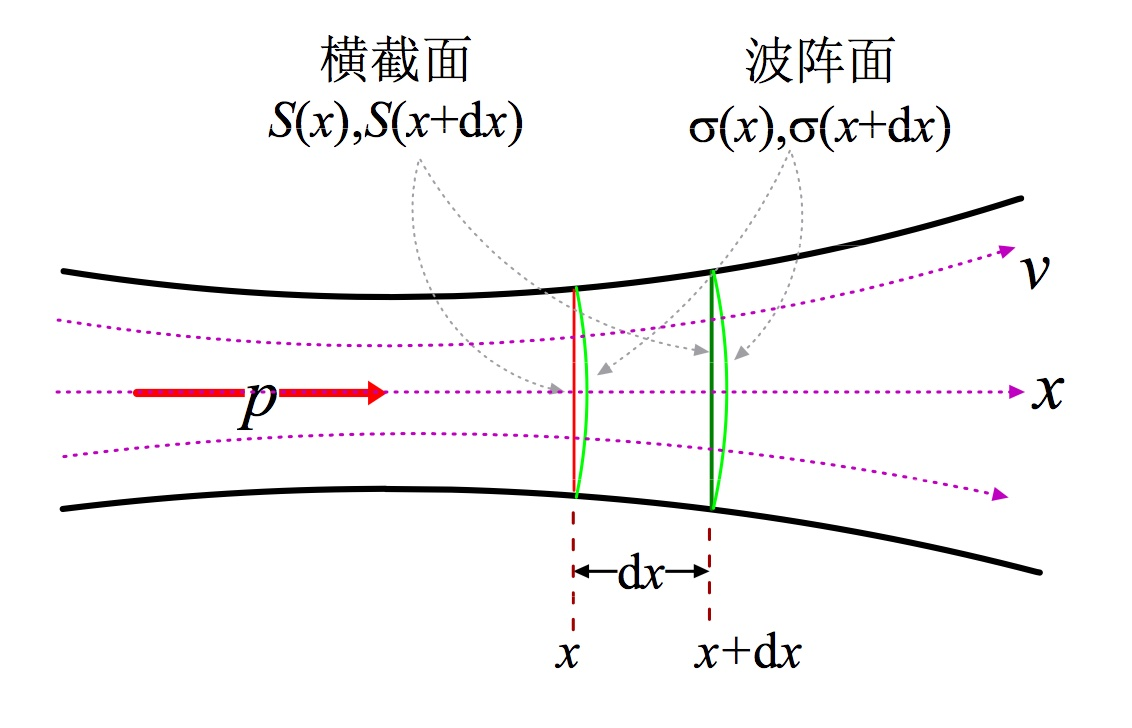
\includegraphics[width=0.7\textwidth]{img/duct/slowlyVaryingPipe.jpg}
	\caption{缓变截面管道模型}
\end{figure}

\subsection{何谓缓变?}
如图(\ref{fig:slowvar_mod})所示的连续变截面管中,管道横截面积和声波波阵面面积皆为管轴向坐标$x$
的函数:
\begin{equation}
	S=S(x)\qc \sigma = \sigma (x)
\end{equation}
因波阵面与管壁正交(壁上法向速度为零),波阵面的面积
$$
\sigma = \iint_\sigma \dd{\sigma} = \iint_\sigma 
\frac{1}{\cos \phi} \dd{S} < \iint_\sigma \frac{1}{\cos\phi_w}\dd{S}
=\frac{S}{\cos\phi_w}$$
其中$\phi$为波阵面法向与管轴的夹角,$\phi_w$为管壁的切角($\phi<\phi_w$)。
于是,
缓变指横截面线度是$x$的缓慢变化的函数,所以
\footnote{如管横截面成圆形,则横截面积的平方正比管半径$R(x)$
	$\tan\phi_w = \dv*{R}{x}$。}
$$
\tan \phi_w \propto \dv{x} \sqrt{S} = O(\eps)
$$
$$\cos \phi_w = \dfrac{1}{\sqrt{1+\tan^2 \phi_w}} = 1+O(\eps^2)
$$
其中$\eps$描述管截面变化的程度。缓变意味着$0<\eps \ll 1$。结果
\begin{equation}
	\label{eq:slowvar_approx}
	\sigma = S\qty[1+O(\eps^2)] \xrightarrow{\ln} \ln \sigma = 
	\ln S+O(\eps^2) \xrightarrow{\dv{x}} \frac1\sigma \dv{\sigma}{x}
	=\frac1S \dv{S}{x}  + O(\eps^2)
\end{equation}

因此,在缓变条件下,$\sigma \approx S$,且$(1/\sigma ) \dv*{\sigma}{x}
\approx (1/S)\dv*{S}{x}$。

\subsection{缓变声管中的声波方程}
回到原坐标$x$,并考察如上图所示由两个相距$\dd{x}$的波阵面所围的小区域$
\Delta V=\sigma \dd{x}$。在此域内对连续性方程作体积分:
$$
0 = \iiint_{\Delta V} \qty[\pdv{\rho}{t} + \div(\rho\vb{v})] \dd{V}
=\iiint_{\Delta V} \pdv{\rho}{t} \dd{V} + \iiint_{\Delta V}\div (\rho \vb{v})
\dd{V}
$$

$$
\xrightarrow{\text{apply Gaussian Theorem}} \dv{t} \qty(\dd{x} \int_{\sigma
(x)} \rho \dd{\bm{\sigma}}) + \int_{\sigma (x+\dd{x})} 
\rho \vb{v}\vdot \dd{\bm{\sigma}} - \int_{\sigma(x)} \rho\vb{v} \vdot \dd
\bm{\sigma} = 0
$$

$$
\xrightarrow{\displaystyle f(x+\dd{x})-f(x) = \dv{f}{x} \dd{x}} 
\dv{t} \qty(\iint_{\sigma(x)} \rho \dd{\bm{\sigma}}) \dd{x}
+\pdv{x} \qty(\iint_{\sigma(x)} \rho \vb{v} \vdot \dd{\bm{\sigma}})\dd x
=0
$$

一般认为,运动与状态量(如密度$\rho$)、以及声学量在波阵面$\sigma$上是常数。
因此,上式中的密度$\rho$可从积分号下取出,而得到管内连续性方程的一维形式:
$$
\pdv{\rho}{t} +\frac1\sigma \pdv{x} (\rho U) = 0\qc \qty(U = \iint_\sigma
\vb{v}\vdot \dd{\bm{\sigma}} = v\sigma) = 0$$
其中$U$为经过波阵面的体积流,为横轴坐标$x$的函数。
因波阵面上速度$v$恒常,垂直波阵面法向,故$U=v\sigma$。
管内运动方程和状态方程一如理想流体者。
经小振幅线性化,连续性方程、运动方程和状态方程依次可近似为:
$$
\begin{cases}
	\displaystyle \pdv{\rho'}{t} +\rho_0 \frac1\sigma \pdv{x}(\sigma v) = 0\\[1em]
\displaystyle \rho_0\pdv{v}{t} = -\pdv{p}{x}\\
p = c_0^2 \rho'
\end{cases}
$$
其中$\rho'$为管内密度扰动量,$\rho_0$为静态密度,$p(x)$为声压。
消去$\rho'$和$v$,得一维声压波动方程,
\begin{equation}
	\label{eq:slowvar_sigmawe}
	\frac1\sigma \pdv{x} \qty[\sigma \pdv{p}{x}]
	-\frac{1}{c_0^2} \pdv[2]{p}{t} =0
\end{equation}
然而,与横截面面积$S$不同,波阵面面积$\sigma$难于获得。
为克服困难,把第一项展开,并应用缓变近似(\ref{eq:slowvar_approx}),
$$
\frac{1}{\sigma}\dv{\sigma}{x} \pdv{p}{x}
+\pdv[2]{p}{x} \approx \frac1S \dv{S}{x} \pdv{p}{x}
+\pdv[2]{p}{x} =\frac1S \pdv{x}(S\pdv{p}{x})$$
如此,方程(\ref{eq:slowvar_sigmawe})可近似为
$$
\frac1S \pdv{x} \qty[S\pdv{p}{x}] -\frac{1}{c_0^2}
\pdv[2]{p}{t} = 0
$$
对于频率$\omega$、波数$k$的时间简谐的声波,此方程简化为
\begin{equation}
	\label{eq:slowvar_helmeq}
	\frac1S \pdv{x}\qty(S\pdv{p}{x}) +k^2p = 0
	\qor
	\pdv[2]{p}{x}+\dv{\ln S}{x} \pdv{p}{x}+k^2p=0
\end{equation}
此乃变系数二阶常微分方程\footnote{此方程与密度非均匀媒质的声波方程(一维)
一致,只要互换$1/S$和$\rho$即可。}。

若把$p$当作「位移」,$x$视为「时间」,$k$视为「固有频率」,方程
(\ref{eq:slowvar_helmeq})岂非质点阻尼振动方程?
只不过,此处阻尼系数$\dv*{\ln S}{x}$是「时间」$x$的函数,且可正可负。
若恰好「阻尼系数」为常数,则方程(\ref{eq:slowvar_helmeq})乃常系数二阶常
微分方程,其解当为人所熟知。
此要求横截面$S$按指数形变化。

若$\dv*{\ln S}{x}$非常数,求解方程(\ref{eq:slowvar_helmeq})殊非易事,需借助
适当的数学方法。
对方程(\ref{eq:slowvar_helmeq})作函数变换:
\begin{equation}
	\label{eq:slowvar_ppsi}
	p(x,t) = \frac{\Psi(x,t)}{R(x)}\qc \qty(R=\sqrt{\frac{S}{S_0}})
\end{equation}
其中$S_0$为某参考面积。波函数$\Psi(x,t)$满足二阶常微分方程:
\begin{equation}
	\label{eq:slowvar_psi}
	\pdv[2]{\Psi}{x} +\qty[k^2-u(x)]\Psi=0
\end{equation}
其不含波函数一阶导数项,而变参数$u(x)$定义为
\begin{equation}
	\label{eq:slowvar_u}
	u(x) \equiv \frac{1}{R(x)} \dv[2]{x} R(x)
\end{equation}
它由管横截面$S$确定。反之,若按设计给定$u(x)$,则可以通过以下二阶常微分方程
\begin{equation}
	\dv[2]{R}{x} - u(x)R=0
\end{equation}
反求符合设计要求的横截面$S(x)$。
方程(\ref{eq:slowvar_psi})是标准的Sturm-Liouville型问题,对于诸多形式的
$u(x)$,存在解析解。
在量子力学中它描述电子穿越势垒(势阱)的量子散射问题,$u(x)$是势函数。

\subsection{典型缓变截面管及其声场}
存在$u(x)$恰为常数的特殊情形,数学处理极其简单,无须求助复杂的数学方法。
记
$$u=\mu^2$$
如此,立刻得到方程(\ref{eq:slowvar_psi})的解:
\begin{equation}
	\label{eq:slowvar_psipm}
	\Psi_\pm = \Psi_{\mathrm{a},\pm} \me^{\mj(\omega t\mp \gamma x)}
	\qc \qty(\gamma = \sqrt{k^2-\mu^2})
\end{equation}
其中「$\pm$」表示分别沿管轴正向和反向传播。
此声波解存在\emph{截止频率}:
$$
f\subt{cutoff} = \frac{\mu c_0}{2\uppi}
$$
当频率低于此频率时,声波是沿管轴指数衰减(增长)的。
欲使$u$恰为此常数,按(\ref{eq:slowvar_u}),$R$只能取如下形式

\begin{subequations}
	\label{eq:slowvar_R}
	\begin{align}
		R & = 1+\frac{x}{x_0}\\
		R& = R_0 \me^{\pm \mu(x-x_0)} \label{eq:slowvar_Rexp} \\
		R&=a\cosh \mu x +b\sinh \mu x \label{eq:slowvar_Rcat}\\
		R& = a\cos \kappa x + b\sin \kappa x\qc (\mu = \mj \kappa)
	\end{align}
\end{subequations}

\begin{itemize}
	\item 锥形($\mu=0$):式中$x_0$为任意常数,表征号筒的扩展程度。
	\item 指数形($\mu>0$):式中$R_0$表征$x=x_0$处号筒的大小。
	\item 悬链线形($\mu>0$):式中$a$和$b$是任意常数。
	\item 正弦形($\mu$是纯虚数)。
\end{itemize}

前三者分别对应于三种典型的声学号筒(horn):锥形、指数形和悬链线形
\footnote{公式(\ref{eq:slowvar_u})中的$u$也可取负的常数值,所得
的$R$呈余弦或正弦形,不过声学上无多大实用意义,故本文不予考虑。}。
把式(\ref{eq:slowvar_psipm})和式(\ref{eq:slowvar_R})代入式(
\ref{eq:slowvar_ppsi}),获得号筒声压通解,再根据谐波速度与声压的一般关系
$$
v=-\frac{1}{\mj k\rho_0c_0} \dv{p}{x}
$$
可获得速度解。

\subsubsection{指数号筒}
不失一般性,设指数号筒函数(\ref{eq:slowvar_Rexp})中的$x_0=0$。
无限长号筒的正向行波解为
\begin{equation}
	\begin{cases}
		p = p\subt{a}\me^{-\mu x+\mj(\omega t \mp \gamma x)}\\
		v = v\subt{a} \me^{-\mu x + \mj (\omega t\mp \gamma x)}
	\end{cases}
	\qc 
	\qty(v\subt{a} = \frac{p\subt{a}}{\rho_0c_0} \me^{-\mj \theta}\qc
	\tan\theta = \frac{\mu}{\gamma})
\end{equation}
号筒任意横截面处的声阻抗
\begin{equation}
	Z\subt{a}(x) = \frac{p}{U} = \frac{p}{S(x)v}
	=\frac{\rho_0c_0}{S(x)} \me^{\mj \theta}
\end{equation}
而声阻抗率是常数。辐射声功率
$$
W = \frac12 \Re(p^* U)|_{x=0}
=\frac{1}{2} \Re(Z\subt{a}|_{x=0}) |U|_{x=0}^2
=\frac12 \rho_0 c_0 S_0 \cos\theta |v\subt{a}|^2
$$
在截止频率处$\theta =\uppi /2$,辐射功率为零\footnote{在截止频率下,$k<\mu$
	声场解为
	$$
	\begin{cases}
		\displaystyle p &\displaystyle =p\subt{a} \me^{\displaystyle
			-\mu x - \sqrt{\mu^2-k^2}x+\mj \omega
	t}\\
	\displaystyle v&\displaystyle =-\frac{1}{\mj k\rho_0c_0} \pdv{p}{x}
	=\frac{\mu+ \sqrt{\mu^2-k^2}}{\mj k} \frac{p}{\rho_0c_0}
	\end{cases}
$$
其声阻抗为
$$Z\subt{a} = \frac{\rho_0c_0}{S(x)} \frac{\mj k}{\mu +\sqrt{\mu^2-k^2}}
=\frac{\rho_0c_0}{S(x)} \frac{\mj \omega}{\omega\subt{cutoff}+\sqrt{\omega\subt{cutoff}^2}
-\omega^2}
=\mj \omega M\subt{a}
$$
$$
\qty(\displaystyle M\subt{a} = \frac{1}{\omega\subt{cutoff}+\sqrt{\omega\subt{cutoff}^2-\omega^2}}
\frac{\rho_0c_0}{S(x)}\qc 
\omega\subt{cutoff}=2\uppi f\subt{cutoff})$$
这是一个声质量抗,声质量为$M\subt{a}$。
}。
当高于截止频率时,$\cos \theta \approx 1$,辐射功率相近乎大活塞的,效率很高
。


\subsubsection{悬链线号筒}
悬链线号筒取式(\ref{eq:slowvar_Rcat})中的$\cosh$型最为合理自然。
同样设$x_0=0$,无限长悬链线号筒的解为:
\begin{equation}
	\begin{cases}
	p&=p\subt{a}\sech \mu x \ \me^{\mj (\omega t-\gamma x)}\\
	\rho_0 c_0 v & = p\subt{a} \sech \mu x\ \frac{
	\cosh (\mu x-\mj \theta)}{\cosh \mu x} \me^{\mj(\omega t-\gamma x)}
	\end{cases}
	\qc 
	\qty(\tan \theta = \frac{\mu}{\gamma })
\end{equation}

\begin{equation}
	\frac{p}{v} = \rho_0c_0 \frac{\cosh \mu x}{\cosh (\mu x-\mj \theta)}
	\xrightarrow{x\to 0} \frac{\rho_0c_0}{\cos\theta}
\end{equation}
在喉口($x=0$)处的声阻抗
$$Z\subt{a}|_{x=0} = \frac{\rho_0c_0}{S_0\cos\theta}$$
为纯声阻,辐射效率很高。辐射声功率
$$W = \frac12 \Re (p^*U) = \frac{1}{2}\frac{\rho_0c_0S_0}{\cos\theta}
|v\subt{a}|^2$$
若喉口振速恒定,则当频率接近截止频率时,辐射功率达无穷大,辐射效率极高。
此特性正与指数号筒相反。

TBD

\chapter{声波的辐射}

% pointfree
\section{自由空间的点声源\\
Point Source of Sound in Free Space}

\emph{摘要}\
点声源犹如质点,是声源的数学抽象。
点声源不仅是理解尺寸小于波长的小型声源辐射的基础,而且是构成一般声辐射的基本元素:任意声源辐射的声场皆可视为点声源辐射声场之叠加。
本文论述点声源辐射的理论及辐射特性。

\subsection{数学模型与声场解}
声源振动激励周围流体而辐射声波。
当存在声源时,流体空间的声场服从有源波动方程。
设$q(\vb{r},t)$是声源在单位时间内单位体积产生的流量,在包围声源体积为$V$的空间之内,源所产生的总流量为
$$
Q(t) = \iiint_V q(\vb{r},t)\dd V
$$

假定空间产生体积流的区域收缩成位于$\vb{r}_0$ 的几何点,同时保持流量$Q$有限且恒定。
为此,在空间位置$\vb{r}_0$单位体积内的流量$q$必趋于无穷大,即:
$$q(\vb{r},t) = Q(t) \delta(\vb{r}-\vb{r}_0)\qc \qty[\iint_V \delta(\vb{r}-\vb{r}_0) \dd V = 1]$$
此即点声源的数学描述。式中$\delta$ 是 Dirac-Delta 函数,在$\vb{r}_0$处奇异,但除点$\vb{r}_0$之外处处为零。
因此,点声源服从如下$\delta$源声波方程:
\begin{equation}
	\laplacian p -\frac1{c_0^2} \pdv[2]{p}{t} = -\rho_0 \dv{Q(t)}{t} \delta (\vb{r}-\vb{r}_0)
	\label{eq:pointfree_delta}
\end{equation}
式中$\rho_0$是球外流体静密度,$c_0$是流体的声速。
如果引入速度势$\Phi$,则流体质点速度$\vb{v}$和声压可表为:
\begin{equation}
	\vb{v}=-\grad \Phi\qc p=\rho_0 \pdv{\Phi}{t}
	\label{}
\end{equation}
 代入方程(\ref{eq:pointfree_delta}),得到速度势$\Phi$满足的波动方程
 \begin{equation}
	 \laplacian \Phi -\frac{1}{c_0^2} \pdv[2]{\Phi}{t} = -Q(t) \delta(\vb{r}-\vb{r}_0)
	 \label{eq:pointfree_Phi}
 \end{equation}

 设有以$\vb{r}_0$ 为球心、半径$a\to 0$的无限小球,包围点源。
 方程(\ref{eq:pointfree_Phi})在此无限小球上的体积分为
\begin{align*}
	\iiint_{|\vb{r}-\vb{r}_0|\leq a}
	\qty(\laplacian \Phi - \frac{1}{c_0^2} \pdv[2]{\Phi}{t} ) \dd V 
	&=
	\iiint_{|\vb{r}-\vb{r}_0|\leq a}
	\qty[-Q(t)\delta(\vb{r}-\vb{r}_0)]\dd V\\
	\iiint_{|\vb{r}-\vb{r}_0|\leq a}
	\div\qty(\grad \Phi)\dd V-\frac{1}{c_0^2} \pdv[2]{t}
	\iiint_{|\vb{r}-\vb{r}_0|\leq a}
	\Phi \dd V&=-Q(t)\\
	\iiint_{|\vb{r}-\vb{r}_0|= a}
	\grad \Phi \vdot \dd \vb{S}
	-\frac{1}{c_0^2} \pdv[2]{t} 
	\iiint_{|\vb{r}-\vb{r}_0|\leq a}
	\Phi \dd V &=-Q(t)
\end{align*} 
 上式第一个积分在所考虑的小球面上的面积分,而第二个体积分是对小球体的体积分,方程右端利用了$\delta$函数的数学性质。

 显然,点声源的声场具有以点源为中心的球对称性:$p=p(r,t)$。
 在源之外,波动方程(\ref{eq:pointfree_delta})是齐次的,其径向向外传播(辐射)的通解为
 \begin{equation}
	 \Phi=\frac1r f\qty(t-\frac{r}{c_0})\qc \qty(r = \norm{\vb{r}-\vb{r}_0})
	 \label{eq:pointfree_PhiSol}
 \end{equation}
 式中,波函数$f(z)$描述所辐射球面波之具体形状,由源决定。
 根据 Euler 运动方程,此速度势场所对应的质点速度$\vb{v}$及其在半径为$a\to0$的、球心位于源点的球面上的面积分为
\begin{align*}
	\vb{v} & = -\grad \Phi = \qty[f\qty(t-\frac{r}{c_0}) +f'\qty(t-\frac{r}{c_0}) \frac{r}{c_0}]\frac{\grad r}{r^2}\\
	\lim_{a\to 0}\oiint_{r=a}\vb{v}\vdot \dd \vb{S} &=
	\lim_{a\to 0} \oiint_{r=a}\qty [f\qty(t-\frac{r}{c_0}) + f'\qty(t-\frac{r}{c_0})\frac{r}{c_0}]\frac{\grad r}{r^2}
	\vdot \dd \vb{S} \\
	&= 4\uppi \lim_{a\to 0} \qty[f\qty(t-\frac{a}{c_0}) +f'\qty(t-\frac{a}{c_0})\frac{a}{c_0}]\\
	& = 4 \uppi f(t)
\end{align*}
其中,函数$f$上的撇号表示对$f(\tau)$的导数:$f'(\tau) = \dv*{f(\tau)}{\tau}$。
显然,根据质量守恒,上式左端的封闭曲面积分等于$Q(t)$。
所以,
\[
f(t)=\frac{Q(t)}{4\uppi}
\]

 由此确定 了$f$的形式。
 代入(\ref{eq:pointfree_PhiSol}),得到点声源的声场解:
 \begin{subequations}
 \begin{align}
	 \Phi & = \frac{1}{4\uppi r}Q\qty(t-\frac{r}{c_0})\\
	 p&= \rho_0 \pdv{\Phi}{t} = \frac{\rho_0}{4\uppi r}Q'\qty(t-\frac{r}{c_0})
 \end{align}
 \label{eq:pointfree_sol}
 \end{subequations}
  若源$Q$是简谐的,频率为$\omega$,源强为$Q\subt{a}$,
  \[Q(t) = Q\subt{a} \me^{\mj \omega t}\]
  则声场解(\ref{eq:pointfree_sol})化为谐波解\footnote{原文为$\Phi(\vb{r},k)$}:
  \begin{subequations}
	  \begin{align}
		  \Phi(\vb{r},\omega) &= \frac{Q\subt{a}}{4\uppi r}\me^{\mj(\omega t -kr)}\\
		  p(\vb{r},\omega) &=\mj k \rho_0 c_0\Phi(\vb{r},\omega)
	  \end{align}
	  \label{}
  \end{subequations}
式中波数$k=\omega/c_0$。
相应的流体径向速度:
\begin{equation}
	v_r=-\pdv{\Phi}{r} = \qty(1+\frac{1}{\mj kr})\mj k \Phi=\qty(1+\frac{1}{\mj kr})\frac{p}{\rho_0c_0}
	\label{eq:pointfree_vr}
\end{equation}
和径向声阻抗率
\begin{align}
	z\subt{s} = \frac{p}{v_r} = \frac{\rho_0c_0}{1+\qty(\mj kr)^{-1}} 
	\xlongrightarrow{kr \gg 1} \rho_0c_0
	\label{eq:pointfree_zs}
\end{align}
 公式(\ref{eq:pointfree_vr})表明,远场($kr\gg 1$)的径向速度和声压近似服从平面波的关系。
 公式(\ref{eq:pointfree_zs})也指出,远场的径向声阻抗率近乎平面波的。

 TBD




% green
\section{点声源与Green函数\\
Point Sources of Sound and Green Functions}

\emph{摘要}\ 
Green函数反映声场的基本结构,也是单位源强的点声源所辐射的声场。
已知Green函数,就可通过积分法获取声场的解析表示。
可见Green函数之于声场之重要性。
然而,在有界媒质空间,因与边界作用之故,点声源辐射问题远较无界空间的复杂。
仅当边界开关及声学性质相对简单的少数情形,才有可能获得封闭的解析解。
多数情形下,最多只能按声场简正模式正交展开的级数解。
本文首先概述基于Green函数的声场积分表示,然后简述若干重要情形的点声源辐射
场(即Green函数)的求解。

\subsection{点声源与Green函数}
设流体空间积分为$V$、边界为$\Sigma$、声特性阻抗率为$\rho_0c_0$,其中在
$\vb{r}_0=(x_0,y_0,z_0)\in V$处存在一点声源,源强为$Q_0$。
点声源犹质点,是数学抽象,其源函数$q(\vb{r})$可表为:
$$q(\vb{r}) = Q_0 \delta(\vb{r}-\vb{r}_0)\qc
\qty(\vb{r},\vb{r}_0\in V\qc Q_0 = \iiint_V q(\vb{r})\dd V)$$
其中$\vb{r}=(x,y,z)\in V$是声场内的观察点的位置,三维Dirac-$\delta$函数
$\delta(\vb{r}-\vb{r}_0)= \delta(x-x_0)\delta(y-y_0)\delta(z-z_0)$。
不妨设此点声源的源强$Q_0=1$,并假设$\Sigma$是阻抗型的边界,故所辐射的声场
速度势$G$满足如下的\emph{有源Helmholtz方程}\footnote{编者注:原文为\emph{
	有源波动方程},有误。}和\emph{边界条件}:
\begin{subequations}
	\begin{align}
		\qty(\laplacian + k^2)G(\vb{r};\vb{r}_0) & =- \delta (\vb{r}-\vb{r}_0)
		\qc \qty(\vb{r},\vb{r}_0\in V) \label{eq:green_Ga}\\
		\qty(\pdv{n} +\mj k \eta )G(\vb{r};\vb{r}_0) & = 0 
		\qc \qty(\b{r},\vb{r}_0\in \Sigma)\label{eq:green_Gb}
	\end{align}
	\label{eq:green_G}
\end{subequations}式中,$k$是声波波数,$\eta$是边界$\Sigma$的声导纳比,由$\Sigma$的法向声阻抗
率$z\subt{n}$定义:$\eta\equiv \rho_0c_0/z\subt{n}$。
$\eta$有两种可能的极端:$\eta=0$的刚性边界和$\eta=\infty$的绝对软边界。
根据方程(\ref{eq:green_Gb})在绝对软边界条件下必有$G=0$,即边界上的
声压为零(稳态场的声压正比于速度势)。
数学上,边值问题(\ref{eq:green_G})的解$G$就是有界空间的Green
函数,它即是观察点$\vb{r}\in V$的函数,也与源点$\vb{r}_0 \in V$有关,故特
写成$G(\vb{r};\vb{r}_0)$的函数形式。
可以证明,\emph{Green函数$G$具有互易性}:
$$G(\vb{r}_2;\vb{r}_1) = G(\vb{r}_1;\vb{r}_2)$$

即位于$\vb{r}_1$的单位源强点源在$\vb{r}_2$处产生的声压(正比于速度势)等于
位于$\vb{r}_2$的单位源强点源在$\vb{r}_1$处产生的声压。
再次强调,尽管Green函数是一个数学概念,但安与点声源的辐射声场建立了直接的
关系:
\begin{equation}
	\Phi (\vb{r}) = Q_0 G(\vb{r};\vb{r}_0)
	\label{eq:green_PhiGreen}
\end{equation}
即,\emph{Green函数 $G$是单位源强($Q_0=1$)的点声源所辐射声场的速度势$\Phi$}
。\footnote{编者注:声压$p$的表达式为:
	$$p(\vb{r}) = \mj \rho_0 \omega \Phi(\vb{r}) = \mj \rho_0 \omega
	Q_0 G(\vb{r};\vb{r}_0)$$}


\subsection{声场的积分表示}
Green函数不仅具有如上所述的物理意义,更重要的是它可用于构造一般声场的解。
一般情形下,空间$V$内的声场既可以是分布式体源$q(\vb{r})$辐射所产生,也可以是
(部分)边界面的振动辐射所产生,如图\ref{fig:green_sketch}所示。
声场的速度势$\Phi(\vb{r})$满足如下\emph{有源波动方程}和\emph{边界条件}:
\begin{subequations}
	\begin{align}
		\qty(\laplacian+k^2)\Phi(\vb{r}) &=-q(\vb{r})\qc 
		\qty[\vb{r} =(x,y,z)\in V]\label{eq:green_Phia} \\
		\qty(\pdv{n} + \mj k \eta )\Phi(\vb{r}) & = u(\vb{r})\qc
		\qty(\vb{r} \in \Sigma)\label{eq:green_Phib}
	\end{align}\label{eq:green_Phi}
\end{subequations}

\begin{figure}
	\centering
	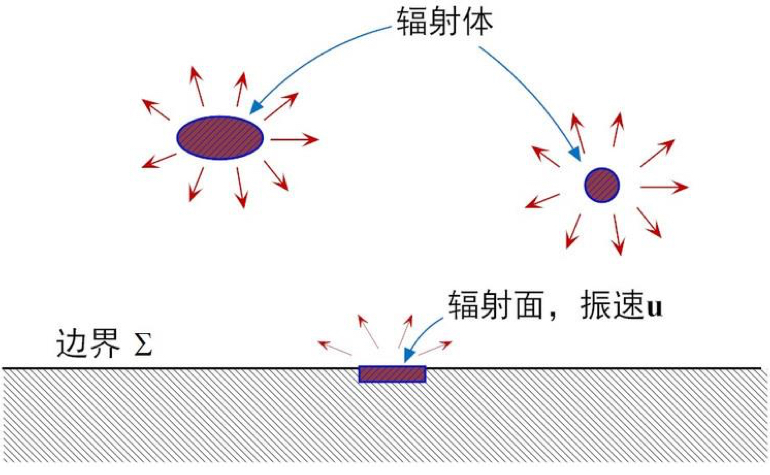
\includegraphics[width=0.7\textwidth]{img/radiation/green_radiationSketch.jpg}
	\caption{体辐射和边界辐射示意图}
	\label{fig:green_sketch}
\end{figure}

根据边界导纳比$\eta$和振速$u$的不同聚会,边界条件(\ref{eq:green_Phib})可以是
以下几种常见类型之一:
\begin{outline}[enumerate]
	\1 刚性边界:$\eta = 0$,且$u = 0$;
	\1 绝对软边界:$\eta = \infty$,即边界上速度势$\Phi=0$;
	\1 给定表面法向振速:$\eta = 0$,但$u\neq 0$;
	\1 阻抗型(非刚性)边界:$\eta \neq 0$,但$u=0$。
\end{outline}

为求解边值问题(\ref{eq:green_Phi}),一般可采用分离变量法先求(\ref{eq:green_Phia})
的通解,然后获得满足边界条件(\ref{eq:green_Phib})的定解。
但除声场空间具有高度对称的极少数情形之外,此种方法笨拙低效。
很多情形下,更行之有效的或许是基于Green函数的积分方法,而求解Green函数问题
(\ref{eq:green_Gb})可作为求解边值问题(\ref{eq:green_Phi})的辅助问题。

用$G(\vb{r};\vb{r}_0)$乘方程(\ref{eq:green_Phia})左右两端,用$\Phi(\vb{r})$
乘以方程(\ref{eq:green_Ga})两端,两者相减后再对其作整个声场空间$V$的体积分,
并利用三维$\delta $函数的积分性质和Gauss定理,得到如下积分方程:
$$
\oiint_\Sigma\qty[G(\vb{r};\vb{r}_0) \pdv{\Phi(\vb{r})}{n} - \Phi(
\vb{r}) \pdv{G(\vb{r};\vb{r}_0)}{n}] \dd \Sigma 
=\Phi(\vb{r}_0) - \iiint_V q(\vb{r}) G(\vb{r};\vb{r}_0) \dd V$$
在此方程中交换$\vb{r}$和$\vb{r}_0$,并利用Green函数的互易性$G(\vb{r};
\vb{r}_0) = G(\vb{r}_0;\vb{r})$,最终得到有源声波方程(\ref{eq:green_Phia})
解的积分表示:\footnote{编者注:使用Einstein求和约定方法,可简化推导。}
\begin{equation}
	\Phi(\vb{r}) = \iiint_V q(\vb{r}_0) G(\vb{r};\vb{r}_0) \dd{V}
	+\oiint_\Sigma \qty[G(\vb{r};\vb{r}_0) \pdv{\Phi(\vb{r}_0)}{n}
	- \Phi(\vb{r}_0) \pdv{G(\vb{r};\vb{r}_0)}{n}]\dd \Sigma
	\qc (\vb{r}\in V)\label{eq:green_kh}
\end{equation}
式中,无论是体积分还是面积分均指对坐标矢量$\vb{r}_0$而言的,$\dd\Sigma$是
$V$在边界$\Sigma$上的面元,\emph{法向指向体积$V$之外}。
公式(\ref{eq:green_kh})形式上给出了声场的积分解。
它表明,有界空间内的声场$\Phi(\vb{r})$是体声源$q$辐射的\emph{直达声}(体
积分项)和\emph{边界反射声}或\emph{辐射声}之和(面积分项)。
边界对声场的影响往往体现在两方面:(1)边界作为振动源主动辐射声波;
(2)边界被动响应声场的作用再影响声场分布。

如果仅存在有限体积的体声源$q$,而无边界$\Sigma$,则上列公式无面积分项。
然而,实际的三维连续振动体声源,总通过自身的边界而向振动体之外空间辐射声波,
故大多可按边界问题处理。
另一方面,若声场空间$V$非封闭,则公式(\ref{eq:green_kh})的面积分尚需包含
无穷远的面积分,例如,半径为$R\to \infty$的球面积分。
如果无穷远处无声波入射,则体积$V$内的声场$\Phi(\vb{r})$尽是$V$内体声源和
边界$\Sigma$产生的,必有$\Phi(\vb{r})\to 0$(熄灭条件),故无穷远边界对声
场的贡献为零,在公式(\ref{eq:green_kh})中可不考虑。
反之,若有来自无穷远处的入射波$\Phi\subt{i}(\vb{r})$,则必须考虑$R\to \infty
$球面的面积分。
其效果等于在公式(\ref{eq:green_kh})中额外加上入射波项$\Phi\subt{i}(\vb{r})$。
此属于\emph{声散射问题},不在本文所论之列。


公式(\ref{eq:green_kh})中尚未考虑到边界条件。
如果Green函数$G$敢与所求声场$\Phi(\vb{r})$所满足的边界条件(\ref{eq:green_Phib})
相应的齐次边界条件(\ref{eq:green_Gb}),则公式(\ref{eq:green_kh})可直接简化为
\begin{equation}
	\Phi(\vb{r}) = \iiint_V q(\vb{r}_0) G(\vb{r};\vb{r}_0) \dd \vb{r}_0
	+\oiint_\Sigma G(\vb{r};\vb{r}_0)u(\vb{r}_0) \dd\Sigma
	\label{eq:green_PhiSimpler}
\end{equation}
它显式地给出了声场的解$\Phi(\vb{r})$。
此公式对$\Sigma$的面积分直接反映了边界辐射对声场的贡献($u$是边界的法向振速
)。
至于边界面的被动反射贡献,已隐含于如此构造的Green函数$G$之中。
如此,一旦已知Green函数,声场速度势的求解仅积分而已矣。
然而,欲求满足与边界条件(\ref{eq:green_Phib})对应的齐次边界条件(
\ref{eq:green_Gb})的Green函数$G$殊非易事,甚至并不比求解原边值问题(
\ref{eq:green_Phi})简单多少。
事实上,Green函数$G$的边界条件不必采取完全与原边界条件(\ref{eq:green_Phib})
对应的齐次形式(\ref{eq:green_Gb})。
在公式(\ref{eq:green_kh})的推导过程中,并未对其中的Green函数$G$的边界条件
作任何限制,甚至可迳取自由空间的Green函数$g$。
是以,Green函数$G$的边界条件的设定存在某种程度的主观随意性。
但是,不同边界条件下所构造的Green函数$G$,不仅其本身的导出或计算难易悬殊,
而且通过公式(\ref{eq:green_kh})计算声场的效率相差万千!
我们的宗旨是尽可能通过公式(\ref{eq:green_kh})高效地求得声场$\Phi(\vb{r})$的
(近似的)解析(或数值)解,而合理选取Green函数$G$的边界条件则可达到事半功
倍之效。

退而求其次,可令Green函数$G$满足更简单的刚性边界条件:
$$\pdv{G}{n}=0\qc \qty(\vb{v}\in\Sigma)$$
如此,公式(\ref{eq:green_kh})面积分中有关Green函数$G$的法向导数项自动为零。
若声场$\Phi(\vb{r})$的边界条件(\ref{eq:green_Phib})恰也有$\eta=0$,则显式解的公式
(\ref{eq:green_PhiSimpler})依然成立;否则,公式(\ref{eq:green_kh})变为
\footnote{编者注:原文积分为$\dd \vb{r}_0$,实际上应该为$\dd^3\vb{r}_0$或
$\dd V$,其中前者更优,因为它强调了是对$\vb{r}_0$而不是$\vb{r}$求积分。}:
\begin{equation}
	\Phi(\vb{r}) = \iiint_V q(\vb{r}_0) G(\vb{r};\vb{r}_0) \dd^3 \vb{r}_0
	+\oiint_\Sigma G(\vb{r};\vb{r}_0) u(\vb{r}_0) \dd \Sigma -\mj
	k\oiint_\Sigma \eta G(\vb{r};\vb{r}_0)\Phi(\vb{r}_0)\dd\Sigma
	\label{eq:green_PhiWithImpedance}
\end{equation}

其中的第二项(面积分)仍是边界主动辐射的贡献,而第三项(面积分)是阻抗型边界
对声场的(被动)反射效应,含特解的速度势函数的边界取值$\Phi(\vb{r}_0)$。
结果,公式(\ref{eq:green_PhiWithImpedance})是积分方程,声场解是\emph{隐式}的
。
隐式解一般可借迭代、变分等计算方法求解。

即使令Green函数满足$G=0$的固定边界条件亦未尝不可,只要能有效地获取简洁的$G$
即可。
若是,则公式(\ref{eq:green_kh})的面积分被积函数仅存包含Green函数法向导数
的第二项。
结果,声场解仍然是隐式的。

可见,积分方法之成败关键在于Green函数$G$的构造合适与否。
因此,求解辅助问题------获取有界空间的Green函数$G$(也就是点源的辐射声场解)
--- --- 成为求解边界问题(\ref{eq:green_Phi})解的数学基础。
而从公式(\ref{eq:green_PhiGreen})可知,所求Green函数,其实就是点声源所辐射的
声场。

\emph{无界空间点声源所辐射的声场}是以源点为中心的球面波,有封闭的解析解。
然而,有界空间因存在边界与声场的相互作用,点声源所辐射声场较为复杂,求解
边值问题(\ref{eq:green_G})殊非易事。
仅在若干简单的情形下,可以轻易求解点源声场的封闭解析表达式,更多的时候或许只能
借助声场简正模式的展开而获得点源声场的渐近级数表示。

TBD


\chapter{声波的吸收}

% viscosity
\section{流体的黏性与声吸收\\
Viscosity and Sound Absorption in Fluids}

\emph{摘要}\
实际流体存在黏性并产生黏滞力,与导热并为声能耗散之因。
黏滞力与流体的应变率成正比。
切变产生切向黏滞力,成为流体运动的内摩擦阻力;容变产生容变黏滞力,使流体的弹性压缩膨胀不可逆。
黏滞不仅造成声能被媒质吸收,也引起某种程度的频散效应。
本文概述流体的黏滞力与应变熟练率的本构关系,及由此导出的黏性流体声波方程,然后简论黏滞所引起的频散与吸收效应。

声吸收是媒质固有的能量损失机制,直接导致声波的耗散。
声吸收之因是媒质固有的黏滞性和导热性。
黏滞和导热是媒质微观分子无规运动的宏观表现,两者共同引起声的宏观机械能不可逆地转化为媒质的热能。
寻常场合声的吸收比较微弱,在有限的时空范围内或许可以忽略不计。
但是,能量的耗散是距离累积性的,长距传播的声波因耗散而导致的声能衰减依然可观。
声的吸收又强烈地依赖于声波频率,频率越高,吸收越强烈。
所以,超声波的吸收多十分显著,不能随便忽略,尤其在具有强烈吸收性的复杂媒质如生物组织中。
此外,在某些特殊情形下,声吸收必须予以考虑。
譬如,微孔管的切向黏滞特别强烈,声波易因强烈的吸收而迅速衰减。
在边界突变附近,声波与不规整边界结构发生强烈的局部相互作用,会产生湍流等复杂振动,使得声能的耗损变得十分强烈。
本文独论流体的黏滞效应所引起的耗散。
至于热导引起的耗散,另当别论。

\subsection{黏滞应力张量}

流体有切变和容变两种黏性,产生切向和容变黏滞力。

\subsubsection{切向黏滞}
切变黏滞存在于有切向速度梯度的流体中,其因在于快慢不同的毗邻流层间发生分子动量交换:慢分子扩散到快层,快分子扩散到慢层。
为阐明之,特考察最简情形。
设有沿$y$方向流动的流体,其速度$v_y$在垂直于流动的$x$方向不均匀,即速度的$y$方向分量$v_y$是$x$的函数:$v_y=v_y(x)$,如下图所示。
\emph{切应变率}
$$\partial_x v_y = \pdv{x} v_y$$
 描述$x$方向单位长度内$y$方向速度的变化程度。
 在任意与流动平行的$x$平面上,左侧流体对右侧流体单位面积上施加正比于切应变率的\emph{切向黏滞应力}:
 $$T_{xy}' = - \eta' \pdv{x} v_y(x)$$
  比例系数$\eta'$称为(切向)\emph{黏滞系数},负号表明黏滞力的方向与切应变率的方向相反。
  应力是单位面积上的力,单位与压强一致,用公制表示是:牛顿/平方米。
  由于应变率的量纲是时间的倒数,故黏滞系数的单位是:牛顿$\times$秒/平方米。
  切黏滞应力$T_{xy}'$中的第一个下标$x$表示黏滞力的作用平面($x$平面),第二个表示黏滞力的方向($y$方向)。

\begin{figure}[h]
	\centering
	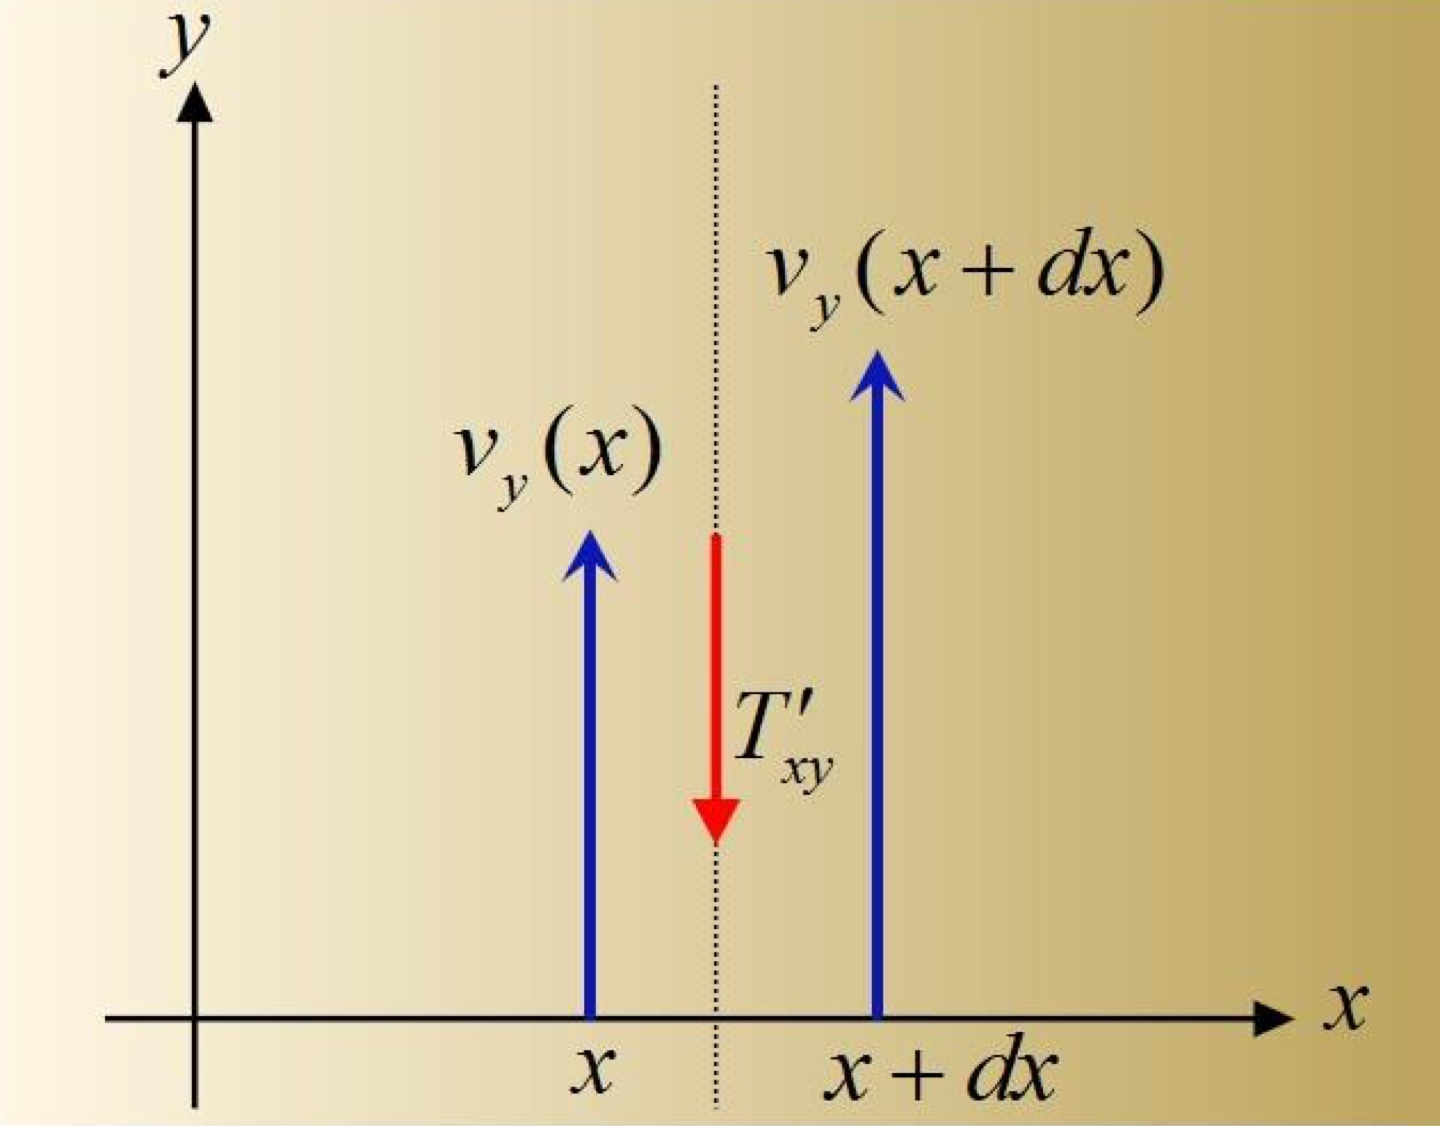
\includegraphics[width=0.5\textwidth]{img/absorption/viscosity_sketch.jpg}
	\caption{流体沿$y$方向流动,其速度在$x$方向存在分布}
	\label{fig:viscosity_sketch}
\end{figure}

 一般,切向黏滞力与速度矢量$\vb{v}=(v_x,v_y,v_z)$的梯度
 $$\grad \vb{v} =\qty{\partial_i v_j\qc i,j = x,y,z}$$
 有关。
 速度的梯度构成应变率张量或矩阵。
 然而,并非速度梯度的所有分量尽引起切黏滞。
 对这些分量作分解
 $$\partial_i v_j = \frac{1}{2}\qty(\partial_i v_j + \partial_j v_i) + \frac12 (\partial_i v_j-\partial_j v_i)$$
  就不难看出,其中包含描述流体纯 旋转的成分;例如,
  $$\partial_x v_y - \partial_y v_x = \pdv{v_y}{x} - \partial{v_x}{y} = \qty(\curl \vb{v})_z$$
  是速度旋度的$z$分量。
  几何分析可以验证,速度旋度之半,
  $$\bm{\Omega} = \frac12 \curl \vb{v}$$
  是流体整体旋转角速度,无关乎切向黏滞,必须在切应变率张量中排除。
  此外,速度散度$\div \vb{v}$表示流体的压缩膨胀体波变化率,对切向黏滞也无贡献,也应从切应变率张量中排除。
  排除了这些成分之后得到的纯\emph{切应变率张量}为

\begin{align*}
	\vb{U} & = \sum_{i,j=(x,y,z)}U_{ij} \vu{e}_i \vu{e}_j\\
	U_{ij} = U_{ji} &= \frac12 \qty(\partial_j v_i + \partial_i v_j) - \frac13 \delta_{ij} \div \vb{v}\qc \qty(\delta_{ij} = \begin{cases}1\qc i=j \\ 0\qc i\neq j\end{cases})
\end{align*}
注意,$U_{xx}+U_{yy}+U_{zz}=0$,恰好排除了体应变的贡献。
\emph{切黏滞应力}是一个\emph{张量},与切应变率张量成正比,
\begin{align}
	\vb{T}' = -2\eta' \vb{U}
	\label{eq:fundamental_shear}
\end{align}
或者,用矩阵表示:
$$ 
\mqty( T_{xx}' & T_{xy}' & T_{xz}' \\
T_{yx}' & T_{yy}' & T_{yz}' \\
T_{zx}' & T_{yz}' & T_{zz}')
=-2\eta'
\mqty(
U_{xx} & U_{xy} & U_{xz}\\
U_{yx} & U_{yy}& U_{yz}\\
U_{zx} & U_{zy} & U_{zz})$$
 因$\vb{U}$对称,切黏滞应力矩阵$\vb{T}'$也对称。


\subsection{容变黏滞}
\emph{容变黏滞}极类于作用于弹簧振子上的摩擦,或者漏气的轮胎,它使流体的压缩膨胀过程不可逆。
容变黏滞产生的原因是在压缩腹背膨胀过程中声的平动机械能转化为分子内部其它自由度的内能,如双原子分子作相对振动的自由度。
单原子分子气体的容变黏滞可以忽略。
与切变黏滞不同,容变黏滞应力正比压缩膨胀率$\div \vb{v}$,方向垂直于流体界面。
数学上,可用三个应力分量描述\emph{容变黏滞应力}:
\begin{align}
	T_{ii}'' = -\eta'' \div \vb{v} \qc \qty(i  = x,y,z)
	\label{eq:fundamental_bulk}
\end{align}
比例系数$\eta''$称为容变黏滞系数。
例如,$T_{xx}''$是作用在$x$平面单位面积上方向沿$x$方向的容变黏滞力。
容变黏滞是各向同性的,所以容变黏滞应力与作用面的方向无关,相应的矩阵是对角的。


\subsection{黏滞应力张量与黏滞力}
综合 公式(\ref{eq:fundamental_shear})和(\ref{eq:fundamental_bulk}),得总的\emph{黏滞应力张量}与\emph{应变率}的关系
\begin{align}
\vb{T}& = \vb{T}' + \vb{T}'' = \sum_{i,j=x,y,z}T_{ij}\vu{e}_i \vu{e}_j\\
T_{ij} & = -\eta' \qty(\partial_j v_i + \partial_i v_j -\frac23 \delta_{ij} \div \vb{v}) - \eta'' \delta_{ij} \div \vb{v} \\
& = \begin{cases}
	 - 2\eta' \partial_i v_i - \qty(\eta'' - \frac23 \eta') \div \vb{v}\qc &(i=j)\\
	-\eta' \qty(\partial_j v_i + \partial_i v_j)\qc &(i\neq j)
\end{cases}
\end{align}
用矩阵表示
$$
\vb{T}= \mqty(T_{xx} & T_{xy} & T_{xz} \\ 
T_{yx} & T_{yy} & T_{yz} \\
T_{zx} & T_{zy} & T_{zz})\qc
\mqty(T_{xy} = T_{yx} \\
T_{xz} =T_{zx} \\
T_{yz} = T_{zy})
$$
它在$x$平面上的三个分量是$\vb{T}_x = (T_{xx}, T_{xy}, T_{xz})$就是该平面上单位面积的黏滞力,如下图所示。
可见,总黏滞力的方向既不垂直于平面,也不与平面相切。
$\vb{T}_x$可以表为张量$\vb{T}$与$x$方向单位矢量$\vu{e}_x=(1,0,0)$的点积
$$ \vb{T}_x = \vb{T} \vdot \vu{e}_x$$
 或者,用矩阵运算表示
$$
\vb{T}_x 
\mqty(T_{xx} \\ T_{xy} \\ T_{xz})=
\mqty(T_{xx} & T_{xy} & T_{xz} \\ 
T_{yx} & T_{yy} & T_{yz} \\
T_{zx} & T_{zy} & T_{zz})\qc
\mqty(T_{xy} = T_{yx} \\
T_{xz} =T_{zx} \\
T_{yz} = T_{zy})
\mqty(1\\0\\0)
$$
同理,可以得到作用在$y$和$z$方向平面上的黏滞力$\vb{T}_y$和$\vb{T}_z$。

\begin{figure}[h]
	\centering
	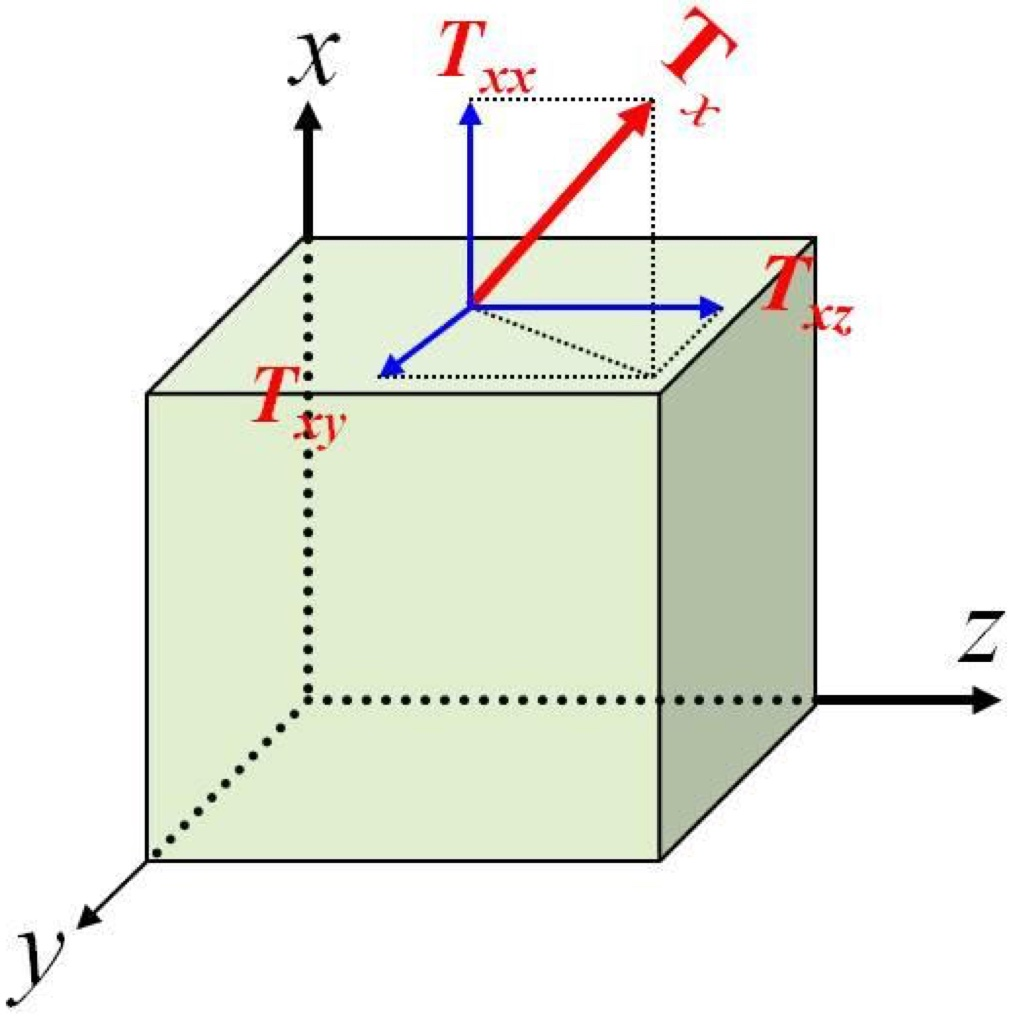
\includegraphics[width=0.4\textwidth]{img/absorption/viscosity_tensor.jpg}
	\caption{作用在$x$平面上的黏滞力$\vb{T}_x$及其分量$T_{xx}, T_{xy}, T_{xz}$}
	\label{fig:fundamental_tensor}
\end{figure}

一般而言,流体内方向单位矢量$\vb{n}$的面积元$\dd S$受到的黏滞力可以表为
$$\dd \vb{F}_\eta = \vb{T} \vdot \qty(\vb{n} \dd S) = \vb{T}\vdot \vb{n} \dd S = \vb{T}_n \dd S$$
所以方向为$\vb{n}$的单位面积受到的黏滞力为
$$\vb{T}_n = \vb{T}\vdot \vb{n}$$
是黏 滞应力张量$\vb{T}$与作用面方向矢量$\vb{n}$的点积。
当然,上式右端也可以表成$\vb{T}$矩阵与$\vb{n}$是矢量的乘积。

\subsection{Navier-Stokes方程}
 体积为$V$的流体,除受到表面流压$P$之外,还受到表面黏滞力,
 $$\oiint \vb{T}_n \dd S = \oiint \vb{T} \vdot (\vb{n}\dd S) = \iiint \div \vb{T} \dd V$$
  其中用到了封闭曲面张量面积分的 Gauss 定理。
  可见,单位体积的流体受到的黏滞力为
 \begin{gather*}
\begin{align*}
	\vb{f}_\eta &= \div \vb{T} = -\eta' \laplacian \vb{v} -\qty(\frac{\eta'}{3}+\eta'')\grad\qty(\div \vb{v})\\
	& = \eta' \curl \curl \vb{v} - \qty(\frac{4}{3}\eta' + \eta'')\grad \qty(\div \vb{v})
\end{align*} \\
\qty[\laplacian \vb{v} = \grad(\div \vb{v}) - \curl \curl \vb{v}]
\end{gather*}
 其中最后等式利用了方括号中的矢量运算关系。
 根据牛顿定律,密度为$\rho$的流体质点的运动方程为
 \begin{align}
	 \rho \dv{\vb{v}}{t} = -\grad P - \vb{f}_\eta = -\grad(P-\eta \div \vb{v}) - \eta' \curl \curl \vb{v} \qc \qty(\eta\equiv \frac43 \eta'+\eta'')
	 \label{eq:absorp_navier}
 \end{align}
 此即 Navier-Stokes 方程,以取代理想流体的 Euler 方程,其中的黏滞系数$\eta$既包含容变黏滞又含切变黏滞。

 对于不可压缩流体,$\div \vb{v} = 0$。方程(\ref{eq:absorp_navier})遂简化为
 $$\rho \dv{\vb{v}}{t} = -\grad P + \eta' \laplacian \vb{v}\qc (\curl \curl \vb{v} = -\laplacian \vb{v})$$
  此即黏性不可压缩流体的运动方程。
  
  不可压缩流体中,惟切变黏滞起作用\footnote{朗道《流体力学》 第二章(中译本)。}。
   对于诸如水等 液体,其运动本质上是不可压缩的,可用此方程描述。
   但是,对于声波而言,媒质 是可压缩的,速度散度非零,必须采用方程(\ref{eq:absorp_navier})\footnote{P. M. Morse \& K. Uno Ingard, Theoretical Acoustics, Princeton University Press. (中译本,1984 年)。}。
   \subsection{黏性流体的声波方程}
 
在小振幅声波情形下,时间全导数可用偏导数近似,Navier-Stokes 方程(\ref{eq:absorp_navier})因此直接线性化为
\begin{align}
	\rho_0 \pdv{\vb{v}}{t} = -\grad (p-\eta \div \vb{v}) - \eta' \curl\curl \vb{v}
	\label{eq:absorp_linear}
\end{align}
式中$\rho_0$为非扰动态的密度。
从此方程立即可知,质点速度的旋度不为零,故而黏性流体的声波运动不再无旋。
开篇已申明,本文不考虑声波过程中因热导而引起的耗散效应。
故而,仍假定绝热状态方程
\begin{align}
	\pdv{p}{t} = -\kappa_s \div \vb{v}
	\label{eq:absorp_state}
\end{align}
成立,其中$\kappa_s$为绝热弹性模量。
方程(\ref{eq:absorp_linear})和(\ref{eq:absorp_state})构成黏性流体声波运动的基本方程组。

\subsubsection{无旋和无散分量}
根据矢量论,任何矢量皆可分解为无旋和无散(有旋)分量之和。
对流体速度矢量$\vb{v}$作此分解
$$\vb{v} = \vb{v}_L + \vb{v}_T$$
$\vb{v}_L$为无旋振速分量,$\vb{v}_T$为无散度振速分量,即
$$\curl \vb{v}_L = 0\qc \div \vb{v}_T = 0$$
无旋分量是纵向(沿传播方向)的振动模式,无散分量是横向(与传播方向垂直)的振动模式。
将此分解代入基本方程(\ref{eq:absorp_linear})和(\ref{eq:absorp_navier}),则可分解为两组方程:无旋

TBD
\end{document}

